% Template for PLoS
% Version 3.1 February 2015
%
% To compile to pdf, run:
% latex plos.template
% bibtex plos.template
% latex plos.template
% latex plos.template
% dvipdf plos.template
%
% % % % % % % % % % % % % % % % % % % % % %
%
% -- IMPORTANT NOTE
%
% This template contains comments intended 
% to minimize problems and delays during our production 
% process. Please follow the template instructions
% whenever possible.
%
% % % % % % % % % % % % % % % % % % % % % % % 
%
% Once your paper is accepted for publication, 
% PLEASE REMOVE ALL TRACKED CHANGES in this file and leave only
% the final text of your manuscript.
%
% There are no restrictions on package use within the LaTeX files except that 
% no packages listed in the template may be deleted.
%
% Please do not include colors or graphics in the text.
%
% Please do not create a heading level below \subsection. For 3rd level headings, use \paragraph{}.
%
% % % % % % % % % % % % % % % % % % % % % % %
%
% -- FIGURES AND TABLES
%
% Please include tables/figure captions directly after the paragraph where they are first cited in the text.
%
% DO NOT INCLUDE GRAPHICS IN YOUR MANUSCRIPT
% - Figures should be uploaded separately from your manuscript file. 
% - Figures generated using LaTeX should be extracted and removed from the PDF before submission. 
% - Figures containing multiple panels/subfigures must be combined into one image file before submission.
% For figure citations, please use "Fig." instead of "Figure".
% See http://www.plosone.org/static/figureGuidelines for PLOS figure guidelines.
%
% Tables should be cell-based and may not contain:
% - tabs/spacing/line breaks within cells to alter layout or alignment
% - vertically-merged cells (no tabular environments within tabular environments, do not use \multirow)
% - colors, shading, or graphic objects
% See http://www.plosone.org/static/figureGuidelines#tables for table guidelines.
%
% For tables that exceed the width of the text column, use the adjustwidth environment as illustrated in the example table in text below.
%
% % % % % % % % % % % % % % % % % % % % % % % %
%
% -- EQUATIONS, MATH SYMBOLS, SUBSCRIPTS, AND SUPERSCRIPTS
%
% IMPORTANT
% Below are a few tips to help format your equations and other special characters according to our specifications. For more tips to help reduce the possibility of formatting errors during conversion, please see our LaTeX guidelines at http://www.plosone.org/static/latexGuidelines
%
% Please be sure to include all portions of an equation in the math environment.
%
% Do not include text that is not math in the math environment. For example, CO2 will be CO\textsubscript{2}.
%
% Please add line breaks to long display equations when possible in order to fit size of the column. 
%
% For inline equations, please do not include punctuation (commas, etc) within the math environment unless this is part of the equation.
%
% % % % % % % % % % % % % % % % % % % % % % % % 
%
% Please contact latex@plos.org with any questions.
%
% % % % % % % % % % % % % % % % % % % % % % % %



\documentclass[10pt,letterpaper]{article}
\usepackage[top=0.85in,left=2.75in,footskip=0.75in]{geometry}

% Use adjustwidth environment to exceed column width (see example table in text)
\usepackage{changepage}

% Use Unicode characters when possible
\usepackage[utf8]{inputenc}

% textcomp package and marvosym package for additional characters
\usepackage{textcomp,marvosym}

% fixltx2e package for \textsubscript
\usepackage{fixltx2e}

% amsmath and amssymb packages, useful for mathematical formulas and symbols
\usepackage{amsmath,amssymb}

% cite package, to clean up citations in the main text. Do not remove.
\usepackage{cite}

% Use nameref to cite supporting information files (see Supporting Information section for more info)
\usepackage{nameref,hyperref}

% line numbers
\usepackage[right]{lineno}

% ligatures disabled
\usepackage{microtype}
\DisableLigatures[f]{encoding = *, family = * }

% rotating package for sideways tables
\usepackage{rotating}

% Remove comment for double spacing
%\usepackage{setspace} 
%\doublespacing

% added by yshira( for using subfigure... this will be not necessary at the time of submission)
\usepackage{graphicx}
\usepackage{subfigure}
\usepackage{bm}
\usepackage{comment}


% Text layout
\raggedright
\setlength{\parindent}{0.5cm}
\textwidth 5.25in 
\textheight 8.75in

% Bold the 'Figure #' in the caption and separate it from the title/caption with a period
% Captions will be left justified
\usepackage[aboveskip=1pt,labelfont=bf,labelsep=period,justification=raggedright,singlelinecheck=off]{caption}

% Use the PLoS provided BiBTeX style
\bibliographystyle{plos2015}

% Remove brackets from numbering in List of References
\makeatletter
\renewcommand{\@biblabel}[1]{\quad#1.}
\makeatother

% Leave date blank
\date{}

% Header and Footer with logo
\usepackage{lastpage,fancyhdr,graphicx}
\usepackage{epstopdf}
\pagestyle{myheadings}
\pagestyle{fancy}
\fancyhf{}
\lhead{\includegraphics[width=2.0in]{PLOS-submission.eps}}
\rfoot{\thepage/\pageref{LastPage}}
\renewcommand{\footrule}{\hrule height 2pt \vspace{2mm}}
\fancyheadoffset[L]{2.25in}
\fancyfootoffset[L]{2.25in}
\lfoot{\sf PLOS}

%% Include all macros below

\newcommand{\lorem}{{\bf LOREM}}
\newcommand{\ipsum}{{\bf IPSUM}}

%% END MACROS SECTION



\begin{document}
\vspace*{0.35in}

% Title must be 250 characters or less.
% Please capitalize all terms in the title except conjunctions, prepositions, and articles.
\begin{flushleft}
{\Large
\textbf\newline{A simple model-based approach to inferring and visualizing cancer mutation signatures}
}
\newline
% Insert author names, affiliations and corresponding author email (do not include titles, positions, or degrees).
\\
Yuichi Shiraishi\textsuperscript{1, *},
Georg Tremmel\textsuperscript{1},
Satoru Miyano\textsuperscript{1},
Matthew Stephens\textsuperscript{2,3,*},
\\
\bigskip
\bf{1} Laboratory of DNA Information Analysis, Human Genome Center, Institute of Medical Science, The University of Tokyo, Tokyo, Japan
\\
\bf{2} Dept. of Human Genetics, University of Chicago, Chicago, Illinois, United States of America
\\
\bf{3} Dept. of Statistics, University of Chicago, Chicago, Illinois, United States of America
\\
\bigskip

% Insert additional author notes using the symbols described below. Insert symbol callouts after author names as necessary.
% 
% Remove or comment out the author notes below if they aren't used.
%
% Primary Equal Contribution Note
% \Yinyang These authors contributed equally to this work.

% Additional Equal Contribution Note
% Also use this double-dagger symbol for special authorship notes, such as senior authorship.
% \ddag These authors also contributed equally to this work.

% Current address notes
% \textcurrency a Insert current address of first author with an address update
% \textcurrency b Insert current address of second author with an address update
% \textcurrency c Insert current address of third author with an address update

% Deceased author note
% \dag Deceased

% Group/Consortium Author Note
% \textpilcrow Membership list can be found in the Acknowledgments section.

% Use the asterisk to denote corresponding authorship and provide email address in note below.
* yshira@hgc.jp; mstephens@uchicago.edu

\end{flushleft}

% Please keep the abstract below 300 words
\section*{Abstract}

Recent advances in sequencing technologies have enabled
the production of
massive amounts of data on somatic mutations from cancer genomes. These data have led to the detection of characteristic patterns of somatic mutations or ``mutation signatures'' at an unprecedented resolution, with the
potential for new insights into
the causes and mechanisms of tumorigenesis.

Here we present new methods for modelling, identifying and visualizing such mutation signatures. Our methods
greatly simplify mutation signature models compared with existing approaches, reducing the number of parameters by orders of magnitude even while increasing the contextual factors (e.g. the number of flanking bases) that are accounted for. This improves both sensitivity and robustness of inferred signatures. We also provide a new intuitive way to visualize the signatures, analogous to the use of sequence logos to visualize transcription factor binding sites. 

We illustrate our new method on somatic mutation data from urothelial carcinoma of the upper urinary tract, and a
larger dataset from 30 diverse cancer types.
The results illustrate several important features
of our methods, including the ability of our new visualization
tool to clearly highlight the key features of each signature,
the improved robustness of signature inferences from small sample sizes, and more detailed inference of signature characteristics such as strand biases and sequence context effects at the base two positions 5' to the mutated site.

%This paragraph is nice, but could be removed if short on words?
% Our work draws on ideas from several tools that are widely used in other contexts. The model for each signature is connected with position weight matrix models for transcription factor binding, and the overall framework is based on probabilistic models that are closely
The overall framework of our work is based on probabilistic models that are closely
connected with ``mixed-membership models'' which are widely used in population genetic admixture analysis, and in machine learning for document clustering. We argue that recognizing these relationships should help improve
understanding of mutation signature extraction problems,
and suggests ways to further improve the statistical methods.

Our methods are implemented in an R package 
{\bf pmsignature} (\url{https://github.com/friend1ws/pmsignature})
and a web application available at \url{https://friend1ws.shinyapps.io/pmsignature_shiny/}.


% Please keep the Author Summary between 150 and 200 words
% Use first person. PLOS ONE authors please skip this step. 
% Author Summary not valid for PLOS ONE submissions.   
\section*{Author Summary}

Somatic (non-inherited) mutations are acquired throughout our lives in cells throughout our body. These mutations
can be caused, for example, by DNA replication errors or exposure to environmental mutagens such as tobacco smoke. 
Some of these mutations can lead to cancer. 

Different cancers, and even different instances of the same
cancer, can show different distinctive patterns of somatic mutations. These distinctive patterns 
have become known as ``mutation signatures".
For example, C $>$ A mutations are frequent in lung caners
whereas C $>$ T and CC $>$ TT mutations are frequent in skin cancers. Each mutation signature may be associated with a specific kind of carcinogen, such as tobacco smoke or ultraviolet light. Identifying mutation signatures
therefore has the potential to identify new carcinogens, and
yield new insights into the mechanisms and causes of cancer, 

In this paper, we introduce new statistical tools
for tackling this important problem. These tools provide more robust and interpretable mutation signatures compared to previous approaches, as we demonstrate by applying them to large-scale cancer genomic data.

\linenumbers

\section*{Introduction}

Cancer is a genomic disease. 
As we lead a life, DNA within our cells acquires random somatic mutations,
mainly caused by DNA replication errors and exposures to mutagens such as chemical substances, radioactivities and inflammatory reactions.  
Although most mutations are harmless (called ``passenger mutations''), 
a small portions of mutations at some specific sites in cancer genes (``driver mutations'') 
%confer growth activities to the cells over other cells,
affect cell growth,
causing autonomous proliferation, tissue invasion, and contributing to oncogenesis \cite{stratton2009cancer}.
Cancer genome studies typically focus on identifying driver mutations, 
to help understand the mechanism of cancer development.
However, passenger mutations can also yield important information, 
because they often show patterns (``mutation signatures'') which 
can provide insights into the forces that cause somatic mutations.
%Classical analyses of mutation patterns have revealed a number of relationships between mutation patterns and carcinogens.
For example, classical studies of mutation patterns
revealed that C $>$ A mutations are abundant in lung cancers in patients with smoking history,
and these are caused by benzo(a)pyrene included in tobacco smoke \cite{pmid12379884}.
Also, C $>$ T and CC $>$ TT  mutations are abundant in ultraviolet-light-associated skin cancers, 
and these are caused by pyrimidine dimers as a result of ultraviolet radiation \cite{pmid15748635}. 

%There were several problems in these classical studies \cite{pmid12379884, pmid15748635}.
The potential for classical studies to yield insights into somatic mutation processes
were limited in several ways.
Due to limited sequencing throughputs, most classical studies 
focused on a few cancer genes, such as TP53,
where high mutation frequencies could be expected. They then
contrasted mutation pattern profiles among different cancer types,
aggregating mutations across multiple individuals within the same cancer type to
yield sufficient mutations for analysis.
However, since many of the mutations in cancer genes are driver mutations causing cell proliferation,
the resultant mutation profiles are a biased representation of the underlying mutation process.
Furthermore, the paucity of mutation data made it effectively impossible to assess variation in mutation patterns among individuals.

Recent advances in high-throughput sequencing provide
new opportunities to investigate sample-by-sample mutation signatures in an unbiased way
using genome-wide somatic mutation data. For example, a large-scale
study using 21 breast cancer samples identified an association of C $>$ [AGT] mutations at TpC sites, 
%Yuichi - is the change association -> excess ok?
%Matthew - actually, what they showed is the relationship between the C>[AGT] mutation at TpC sites and kataegis.
which was later proved to be caused by APOBEC protein family \cite{pmid23389445, pmid23852168, pmid23852170}, 
and a novel phenomenon called {\it kataegis} \cite{pmid22608084}. 
Moreover, a landmark study of 7,034 primary cancer samples, representing 30 different cancer classes, has provided the first large-scale overview of mutation signatures across a large number of cancer types \cite{pmid23945592}. This has lead to great hopes that detection of novel mutation signatures and associated mutagens can lead to identification of novel mutagens and prevention of cancer.

To make the most of these opportunities requires the development
of efficient and effective statistical methods for analyzing
mutation signatures in vast amounts of somatic mutation data.
Current statistical approaches \cite{pmid23318258,pmid23628380}, 
%based on nonnegative matrix factorization (NMF, \cite{pmid10548103}) and Poisson models
are an excellent starting point, 
and have helped generate the new insights noted above.
However, we argue here that these existing methods 
have two important limitations, caused by the fact that they
use an unconstrained model for each ``mutation signature."
First, although using an unconstrained model might appear to be a good thing in terms of flexibility, 
in practice it can actually reduce flexibility, because
the price of using an unconstrained model is that one must limit 
the domain of mutation signatures considered. 
For example, most recent analyses of mutation signatures
consider only the immediate flanking 5' and 3' bases of each substitution to be part of
the signature, even though it is known that more distal bases -- and particularly the
next flanking base on each side -- can contain important contextual information
\cite{pmid9683596}. These recent analyses take this approach because, in the unconstrained model,
incorporating the more distal bases into the signature very substantially increases the number of parameters, making estimated mutation signatures unstable.
Secondly, and just as important, the unconstrained model means
that each signature is a probability distribution in a high-dimensional
parameter space, which can make signatures difficult to interpret.

In this paper, we present a novel probabilistic approach 
to mutation signature modelling that addresses these limitations.
In brief, we first simplify the modelling of mutation signatures by decomposing them into separate ``mutation features".
For example, the substitution type is one feature; flanking bases are each another feature. We then exploit this 
decomposition by using a probabilistic model for signatures that assumes independence across features. This approach substantially reduces the number of parameters associated with
each signature, greatly facilitating the incorporation of additional relevant sequence context. 
For example, our approach can
incorporate both the two bases
3' and 5' of the substitution, and transcription strand biases using only 18 parameters
per signature, compared with 3071 parameters per signature with current approaches. We demonstrate the benefits of this simplification in data analyses. These benefits include: more stable estimation of signatures from smaller samples, 
refinement of the detail and resolution of many mutation signatures, and, possibly, identification of novel signatures.

Assuming independence among features in a signature may initially seem unnatural. However, its use here is analogous  ``position weight matrix models" which have been highly
successful 
for modelling transcription factor binding motifs.
Indeed, an important second contribution of
our paper is to provide intuitive visual representations for mutation signatures,
analogous to the ``sequence logos" used for visualizing binding motifs.
Finally, we also highlight the close connection
between mutation signature models and the ``mixed-membership models'',
also known as``admixture models" \cite{pmid10835412} or ``latent Dirichlet allocation''
models \cite{Blei:2003} that are widely used in population genetics 
and document clustering applications.
These connections should be helpful for future elaboration of 
computational and statistical methods for cancer mutation signature detection. 



%The second point is that we adopt the framework of ``mixed membership models'' for the mutation signature problem. The mixed memberships model are basically clustering methods, but allowing that each individual can have multiple clusters, and widely used in many different fields such as population structure classification in population genetics \cite{pmid10835412} and document classification problems in machine learning \cite{Blei:2003}. This models are also shown to be closely related to nonnegative matrix factorization \cite{ding2008equivalence}.


% In addition, even though it has not been widely discussed, 
% the problem of identifying mutation signatures is closely related to "mixed-membership models,''
% that is widely used in other field such as ``population admixture'' models \cite{pmid10835412} in the analysis of population structure, 
% and the ``latent dirichlet allocation'' (LDA) model for document clustering \cite{Blei:2003}.
% In this paper, we explicitly show the relationships between the proposed model and the mixed-membership models and discuss the relationships,
% which we believe will be highly helpful for future elaboration of the statistical method for mutation signature extraction problems.

Software implementing the proposed methods is available in an R package 
{\bf pmsignature} ({\bf p}robabilistic {\bf m}utation signature),
at \url{https://github.com/friend1ws/pmsignature}.
The core part of the estimation process is implemented in C++ by way of the Rcpp package \cite{eddelbuettel2011rcpp},
which enables handling millions of somatic mutations from thousands of cancer genomes using a standard desktop computer.
In addition, a web-based application of our method is available at 
\url{https://friend1ws.shinyapps.io/pmsignature_shiny/}.


% Results and Discussion can be combined.
% \section*{Methods Overview}
\section{Result}


\subsection*{New model for mutation signatures}

The term ``mutation signature'' is used to describe a characteristic mutational pattern observed in cancer genomes. Such patterns are often related to carcinogens (e.g., frequent C $>$ A mutations in lung cancers with smoking histories).

What constitutes a mutational pattern varies among papers.
The simplest approach is to consider 6 possible mutation patterns, corresponding to
6 possible substitution patterns (C$>$A, C$>$G, C$>$T, T$>$A, T$>$C, T$>$G; the original base is often fixed to C or T to remove redundancy of taking complementary strands).
However, in practice we know that DNA context of a substitution is often important, and so it is common to go the next level of complexity, and include the immediate 5' and 3' flanking bases in the mutation pattern.
This results in 96 (6 $\times$ 4 $\times$ 4) patterns. 
Further incorporating the strand (plus or minus) of each substitution extends this to 192 patterns \cite{pmid23945592, pmid23318258}. 


% In this paper, we call the factors composing mutation patterns (such as substitution patterns, adjacent bases and transcriptional strand) 
% as ``mutation features.''

Mathematically, mutation signatures have previously been characterized using an unconstrained distribution over mutation patterns \cite{pmid23318258,pmid23628380}. Thus, if the number of mutation patterns considered is $M$ then each
mutation signature is characterized by a probability vector
of length $M$ (which must sum to 1, so $M-1$ parameters). 
A problem with this approach is that
it requires a large number of parameters per mutation signature. As noted above,
even accounting only for immediately flanking bases 
gives $M=96$.  Furthermore, $M$ increases exponentially if we try to account for additional context: to take account of up to $n$ bases 5' and 3' to the mutated site 
(henceforth referred to as the $-n$ position and the $+n$ position, respectively) gives $M=6 \times 4^{2n}$. 
Having a large number of parameters per signature causes
two important problems: i) estimates of signature parameters can become statistically unstable; ii) signatures can become
difficult to interpret.



% On the other hand, the mutation rates are mostly below 10 per Mb \cite{pmid23945592},
% (where about 30,000 mutations are expected in entire genomic regions).
% Therefore, considering even $\pm 2$ positions and substitution patterns (1535 parameters)
% can cause instability in parameter estimation. 


% On the other hand, observing the mutation signatures detected in the previous studies, 
% many mutation signatures have clear characteristics such as:
% \begin{itemize}
% \item 
% A certain value of mutation features is often dominant in many known mutation signatures. 
% For example, the base T is highly dominant at the $-1$ position in the APOBEC signature, 
% and C $>$ T substitution is highly dominant in the ultraviolet signature \cite{pmid23945592} (see Figure \ref{APOBEC_nature2013_sig}). 

% \item
% Proportional relationships among mutation features are often observed in many signatures as shown in the APOBEC signature, 
% where the frequencies of bases at the $+1$ position are largely proportional across 3 major substitution patterns C$>$T, C$>$G and C$>$A,
% showing consistent tendencies  (A and T bases are more frequent than C and G bases).

% \end{itemize} 

% These characteristics imply that the parameter spaces of mutation signatures can be degenerated to lower dimensional spaces in many cases, 
% and we can potentially reduce the number of parameters by imposing additional restrictions. 

The first contribution of this paper is to suggest
a more parsimonious approach to modelling 
mutation signatures, with the benefit of producing both more stable estimates and more easily-interpretable signatures.
In brief, we substantially reduce the number of parameters
per signature by breaking each mutation pattern into 
``features", and assuming independence
across mutation features. For example, consider
the case where a mutation pattern is defined by the substitution and its two flanking bases. We break this into three features (substitution,
3' base, 5' base), and characterize each mutation
signature by a probability distribution for each feature
(which, by our independence assumption, are multiplied
together to define a distribution on mutation patterns). Since the number of possible values for each feature is 6, 4, and 4 respectively this requires $5+3+3=11$ parameters instead of $96-1=95$ parameters. Furthermore, extending this model to account for $\pm n$ neighboring bases requires only $5 + 6n$ parameters instead of $6 \times 4^{2n} - 1$. For example,
 considering $\pm 2$ positions requires 17 parameters
 instead of 1535. Finally, incorporating
transcription strand as an additional feature adds just one parameter, instead of doubling the number of parameters.

Since the aim of a mutation signature is, in some ways, to capture dependencies among features, the independence assumption may seem counter-intuitive. However, the
idea is exactly analogous to the use of a ``position weight matrix" (PWM) to represent motifs in sequence data. In this
analogy, a motif is analogous to a mutation signature, and each location in the motif is analogous to a ``feature". Just as we use a probability vector for each feature, a PWM defines a probability vector for each location in a motif,
and these probabilities at each location can be multiplied together to yield a probability
distribution on sequences.
Even though a PWM cannot capture complex 
higher-order dependencies, some of which likely do exist in practice, it has been a highly successful tool for motif
analysis - likely because it can capture the most important characteristics of transcription factor binding sites 
(that some locations will show strong preference for a particular base, whereas others will not), and also
because it can be represented in an easily-interpretable way via sequencing logos \cite{pmid2172928}.
For similar reasons -- in addition to the empirical
demonstrations we present later -- we believe our mutation signature representation will prove useful for mutation signature analysis. 

Fig. 1 illustrates the way that our new representation of signatures can simply capture
a previously-identified signature \cite{pmid25362482, pmid23318258} and provides
an easily-interpretable visualization of the signature 
that is analogous to  sequencing logos \cite{pmid2172928}.
We particularly note how the key elements of this mutation signature are more immediately visually apparent than with visualizations of the full vector of probabilities used by existing approaches.

\begin{figure}[h]

\caption{{\bf Examples of visualizations and parameter values for the mutation signatures of the unconstrained (full) model and our independent model, 
where substitution patterns, two 5' and 3' bases and transcription strand direction are considered as mutation features.}
(A) The barplots are divided by 6 substitution patterns and transcription strand direction.
In each division, 256 bars show joint probabilities of up to two base 5' and 3' bases
(ApApNpApA, ApApNpApC, ApApNpApG, ApApNpApT, $\cdots$, TpTpNpTpT).
(B, C) An example mutation signature representation and parameter values from our independent model, where mutation features (substitution patterns, two 5' and 3' bases and strand direction) 
are assumed to be independent ($L=6$, $\bm{M} = (6, 4, 4, 4, 4, 2)$).
In the bottom five rectangles, the width of each box represents the frequencies of bases (A, C, G and T) at the substitution and flanking site. 
To highlight the most informative flanking sites, the heights of flanking site boxes are scaled by ($1 + 0.5 \times \log \sum_{n = A,C,G,T} f_n^2$, where $f_n$ is the parameter for each base), which can be interpreted as ($1 - 0.5 \times \text{R\'enyi entropy}$) \cite{rrnyi1961measures}. This is analogous to the information content scaling used in sequencing logos.
In the top rectangle, the height of each box represents the conditional frequencies of mutated bases for each original base (C and T).
In the upper right, the height of the $+$ box represents the frequencies of mutations in the coding strand (or the plus strand, the sense strand and the untranscribed strand)
whose nucleotide sequences directly corresponds to mRNA, 
whereas the height of $-$ box represents those in the template strand (or the minus strand, the antisense strand, the transcribed strand and the noncoding strand)
whose sequences are copied during the synthesis of mRNA.
}
\label{mutSig_example}

\end{figure}

% Let's consider putting this in the discussion:
% Although most mutation signatures show proportional relationships among mutation features, 
% a few signatures seem to violate proportional relationships and cannot be explained by independent models. 
% For example, the pol $\epsilon$ mutation signature \cite{pmid23945592} (see Figure \ref{POLE_nature2013_sig}) puts strong probability masses 
% on just two pattern TpCpT $>$ TpApT and TpCpG $>$ TpTpG, 
% and the frequencies of substitution patterns and bases at the $+1$ positions are not proportional unlike the APOBEC signature.
% However, by using multiple mutation signatures, we can represent this phenomenon even under the independence assumption.

%In this paper, we focus on substitution patterns, flanking bases (up to the $\pm 2$ positions) and transcribed directions as contextual factors of mutation patterns.

% \subsection*{Mathematical specification, and connection with mixed-membership models}
\subsection*{An overview of mathematical specification of mutation signatures and the generative model of somatic mutations}

% yshira20150421 I think the title of the section should change (because this is not "detail").

Suppose each somatic mutation has $L$ mutation features, $\bm{m} = (m_1, m_2, \cdots, m_L)$, 
where each $m_l$ can take $M_l$ discrete values. Also, let $\bm{M} := (M_1, \cdots, M_L)$.
For example, when taking account of 6 substitution patterns and $\pm 2$ flanking sites,
$\bm{M} = (6, 4, 4, 4, 4)$.
See S1 Table for other examples.

Suppose we have observed mutations in $I$ sampled cancer genomes, and let $J_i$ denote the number of observed mutations in the $i$-th cancer genome.
Further, let
$\bm{x}_{i, j} = (x_{i, j, 1}, \cdots, x_{i, j, L}), (i = 1, \cdots, I, j = 1, \cdots, J_i)$ denote the observed mutation feature vector for the $j$-th mutation of $i$-th cancer genome,
where $x_{i, j, l} \in \{1, \cdots, M_l \}$.

Our model assumes that each mutation arose from one of $K$ possible mutation signatures. Each cancer sample has its own characteristic proportion of mutations of each signature type (which might depend on lifestyle, genetic differences, etc.).
We let $q_{i,k}$ denote the proportion of signature $k$ in sample $i$, so $\bm{q}_i = (q_{i,1}, q_{i,2}, \cdots, q_{i, K}) \in \Delta^K,  (i = 1, \cdots, I)$ where $\Delta^S = \{ (t_1, \cdots, t_S) : t_s \geq 0 \, \forall s, \sum_{s=1}^S t_s = 1 \}$ denotes the S-dimensional simplex of non-negative vectors summing to 1.
Further, each mutation signature is characterized by parameter vectors $\bm{F}_k := (\bm{f}_{k,1},\dots,\bm{f}_{k,L})$, where \bm{$f}_{k,l}$ is a probability vector for
the $l$-th feature in the $k$-th signature.
That is,  $\bm{f}_{k, l} = (f_{k, l, 1}, \cdots, f_{k, l, M_l }) \in \Delta^{M_l}$.

Our generative model for the observed mutations $\{ \bm{x}_{i,j} \}$ in each
cancer sample can now be described as a two-step process.
\begin{enumerate}
\item
Generate $z_{i,j} \sim \text{Multinomial} (\bm{q}_m)$, where $z_{i,j} \in \{1,\cdots,K \}$ denotes the (unobserved) underlying mutation signature that caused the $j$-th mutation in the $i$-th sample.
\item 
For each $l (= 1, \cdots, L)$, generate $x_{i,j,l} \sim \text{Multinomial}(\bm{f}_{z_{i,j},l})$.
Thus, 
\begin{equation}
\Pr(x_{i,j,l} = m | z_{i,j}=k) = f_{k,l,m} 
\end{equation}
\end{enumerate}

This generative model is summarized in Fig. \ref{methodOverview}.
This model is essentially a ``mixed-membership model", also known as an ``admixture model" \cite{pmid10835412} or ``latent Dirichlet allocation" \cite{Blei:2003}. For example,
the membership proportions for each sample are analogous to admixture proportions in an admixture model; the mutation signatures are analogous to 
populations, and the mutation signature-specific parameters are analogous to population-specific allele frequencies.

The key parameters in this model
are the membership proportions for each sample, $\bm{q}_i$, and the mutation signature parameters, $\bm{F}_k$. 
We estimate these parameters by maximizing likelihood using an EM algorithm. 
A simulation study demonstrates that the estimation method can reproduce the mutation signature very accurately 
provided enough mutations and samples are available (see S1 Text). 
See Methods for more detailed models, parameter estimation, further discussion on relationships with mixed membership models, how to select $K$, etc.


\begin{figure}[h]
% 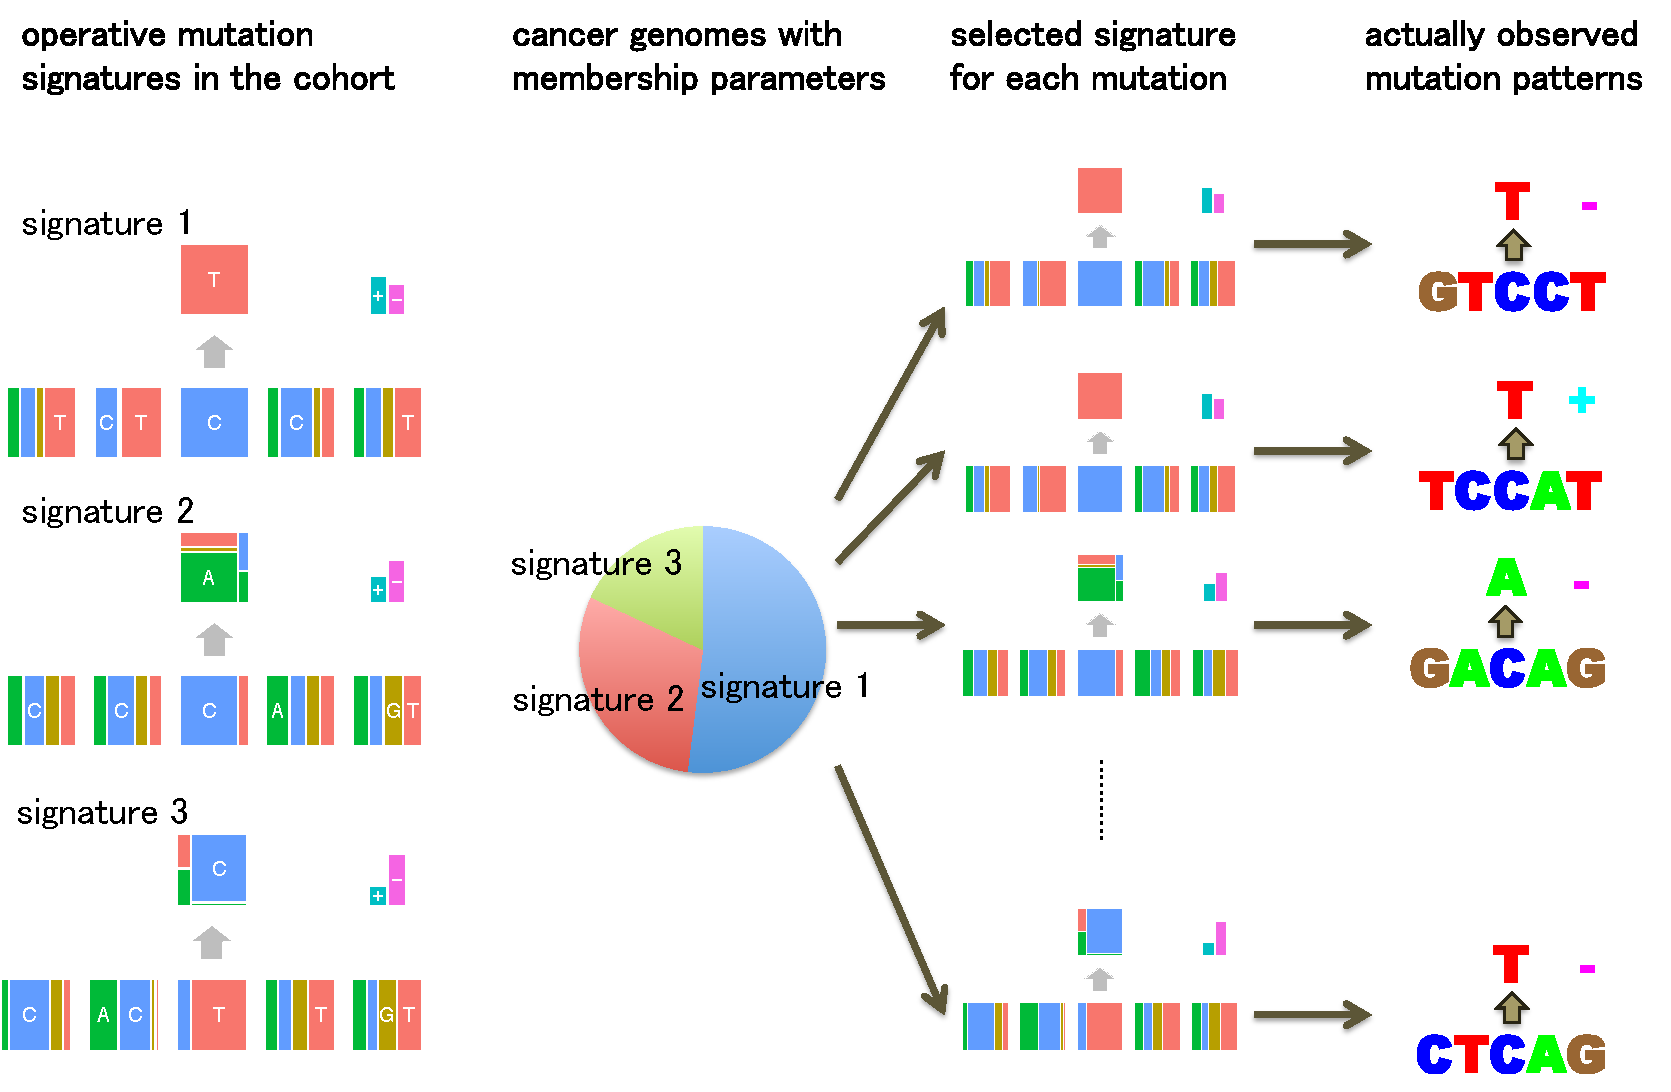
\includegraphics[width=450pt]{methodOverview.pdf}
\caption{{\bf An overview of the generative model of somatic mutations proposed in this paper.} 
Suppose there are three types of mutation sources (mutation signatures) such as ultraviolet, tobacco smoking chemicals and transcription coupled repairs.
Each cancer genome has ratios showing which types of mutation sources are contributing to its mutations (membership parameters).
The generative model of the pattern of each mutation is:
first, one of the mutation signatures is chosen according to the membership parameter.
Second, each mutation feature such as substitution patterns and flanking bases is generated 
by the corresponding multinomial distributions for the selected mutation signature.
}
\label{methodOverview}
\end{figure}


% yshira20150421 I tried to mention about background signature very shortly in the main text as above. 
% But I feel the necessity of further discussion.
The intrinsic composition of genome sequence, if unaccounted for, can undesirably influence estimated mutation signatures.
For example, since the di-nucleotide CpG is underrepresented in most genomic regions (other than promoters), 
a signature with substitutions from a C base can have weaker signals of G base at the $+1$ position.
In previous work \cite{pmid23628380}, this background problem was dealt by explicitly incorporating ``mutation opportunity'' coefficients into the model.
Here, to reduce the influences of intrinsic sequence composition on our signature estimates, we introduce a special ``background signature"
$\{ \bm{F}_{0} \} \in \Delta^{M_1 \times \cdots \times M_L}$, 
which is designed to capture biases in intrinsic genome sequence composition and is calculated from the composition of consecutive nucleotides of the human genome sequence 
(See Methods for the detail).


% Results and Discussion can be combined.
% \section*{Results}


\subsection*{Robustness experiments using cancer genomes from urothelial carcinoma of the upper urinary tract}

Here we compare our new ``independent model'' for 
mutation signatures, which assumes independence
among mutation features,
with the ``full model'', which corresponds to existing approaches. We compare mutation signatures obtained by the two approaches and investigate the robustness of each approach by down-sampling experiments.

The data consist of 14717 somatic substitutions 
collected from a study of 26 urothelial carcinomas of the upper urinary tract (UCUT) \cite{pmid23926200}.
The original study identified a novel mutation signature in these data: 
T $>$ A substitutions at CpTpG sites with a strong transcription strand specificity caused by aristolochic acids (AA).

We consider a mutation pattern to consist of the substitution pattern, the $\pm 2$ flanking bases, and the transcription strand direction. Thus each signature is characterized by 18 parameters in our independent model, and by 3071 parameters in the full model. After analyzing the data with various number of mutation signatures $K$,
we selected $K=3$ signatures for these analyses (see S2 Text).


The inferred APOBEC signature under the independent model
shows a clear depletion of G base at the $-2$ position,
which is consistent to the previous study \cite{pmid23318258} and results in the next subsection (Figs. 3A and 3B).
In contrast, for the full model, this tendency is rather mild (Figs. 3C, 3D and S1).
The inferred AA mutation signature has no clear characteristics at the $-2$ position.
These results suggest that our independent model has the potential
to identify signatures in more detail and with less data than existing approaches based on the full model.

\begin{figure}[h]
\caption{{\bf The mutation signatures for the UCUT data, and the results of down-sampling experiments.}
3072 elements in the full model mutation signatures were shown divided by 6 substitution patterns and strand directions.
(A, B) APOBEC and AA signature for the independent model.
(C, D) APOBEC and AA signature for the full model.
(E, F) APOBEC and AA signature stability (the mean cosine similarity for each down-sampling ratio).}
\label{UCUT}
\end{figure}

To investigate this further we performed down-sampling experiments.
Using the mutation signatures obtained using all 14717 substitutions as a gold standard, 
we assessed performance of the proposed method on down-sampled data consisting of $r\%$ of the original data, where  $r=(1\%, 2.5\%, 5\%, 10\%, 25\%, 50\%)$.
To measure robustness we used the cosine similarity on the 
full dimensional vector space, which allows comparison between the full model and the independent model.
We repeated each down-sampling experiment 100 times for each model.

% For measuring the deviations of the mutation signature, the cosine similarity was used on the $\prod_{l=1}^L M_l$ dimensional vector space $f_{i, \bm{m}} = \prod_{l=1}^L f_{k,l,m_l}$,

The results (Figs. 3E and 3F)
confirm that the results of the independent model 
are substantially more robust to reductions in data size than the full model. Indeed, mutation signatures inferred using the independent model with only 10\% of the data 
remain highly similar to the signatures inferred from the full data; by comparison the full model shows a much larger drop-off in similarity, especially in the APOBEC signature where even using 50\% of the data gives a substantial drop-off in similarity. Both methods found the AA signature 
easier to recover than the APOBEC signature.
We believe that this is because the number of T $>$ A substitutions at GpTpC sites are far more frequent in this dataset.



\subsection*{Application to somatic mutation data of 30 cancer types}
 
To provide a more comprehensive practical illustration of
our method, we applied it to somatic mutation data from 30 cancer types \cite{pmid23945592}.
We applied the method to each cancer type separately to assess similarity of estimated signatures across cancer types.
For each cancer type we selected the number of signatures $K$ by fitting the model with increasing $K$ and examining the log-likelihood, bootstrap errors, and correlation of membership parameters.
The selected values of $K$ are given in S2 Table.
Also, we simply removed somatic mutations located in an intergenic region to include transcription strand biases as mutation features.
Finally, we merged similar mutation signatures across different cancer types 
(when their Frobenius Distance were $<$ $0.6$). 
% XXX WHAT KIND OF CLUSTERING?
 % (see Supplementary Material for the values of the log-likelihoods and bootstrap errors for each cancer type).



Figs. \ref{nature2013_sig_summary} and \ref{nature2013_sig_member} summarise the results.
In total, we identified 27 mutation signatures.
Many of these signatures show reassuring similarities with
signatures identified in previous studies. However
signatures from our independence model, because of its ability to effectively
and parsimoniously deal with both $\pm2$ flanking
base context and strand bias, are often more refined, highlighting additional details or features not previously evident. By comparing the composition of nucleotides and cancer types exhibiting the signatures with results of previous studies, we were able to associate many of the detected signatures with known mutational processes.
In addition, as we reviewed these signatures
and compared them with previous work, we noticed connections
that, while not directly related to our new model, appear
novel and noteworthy. The remainder of this section
provides a comprehensive discussion of these findings.

\begin{figure}[h]
\centering
% 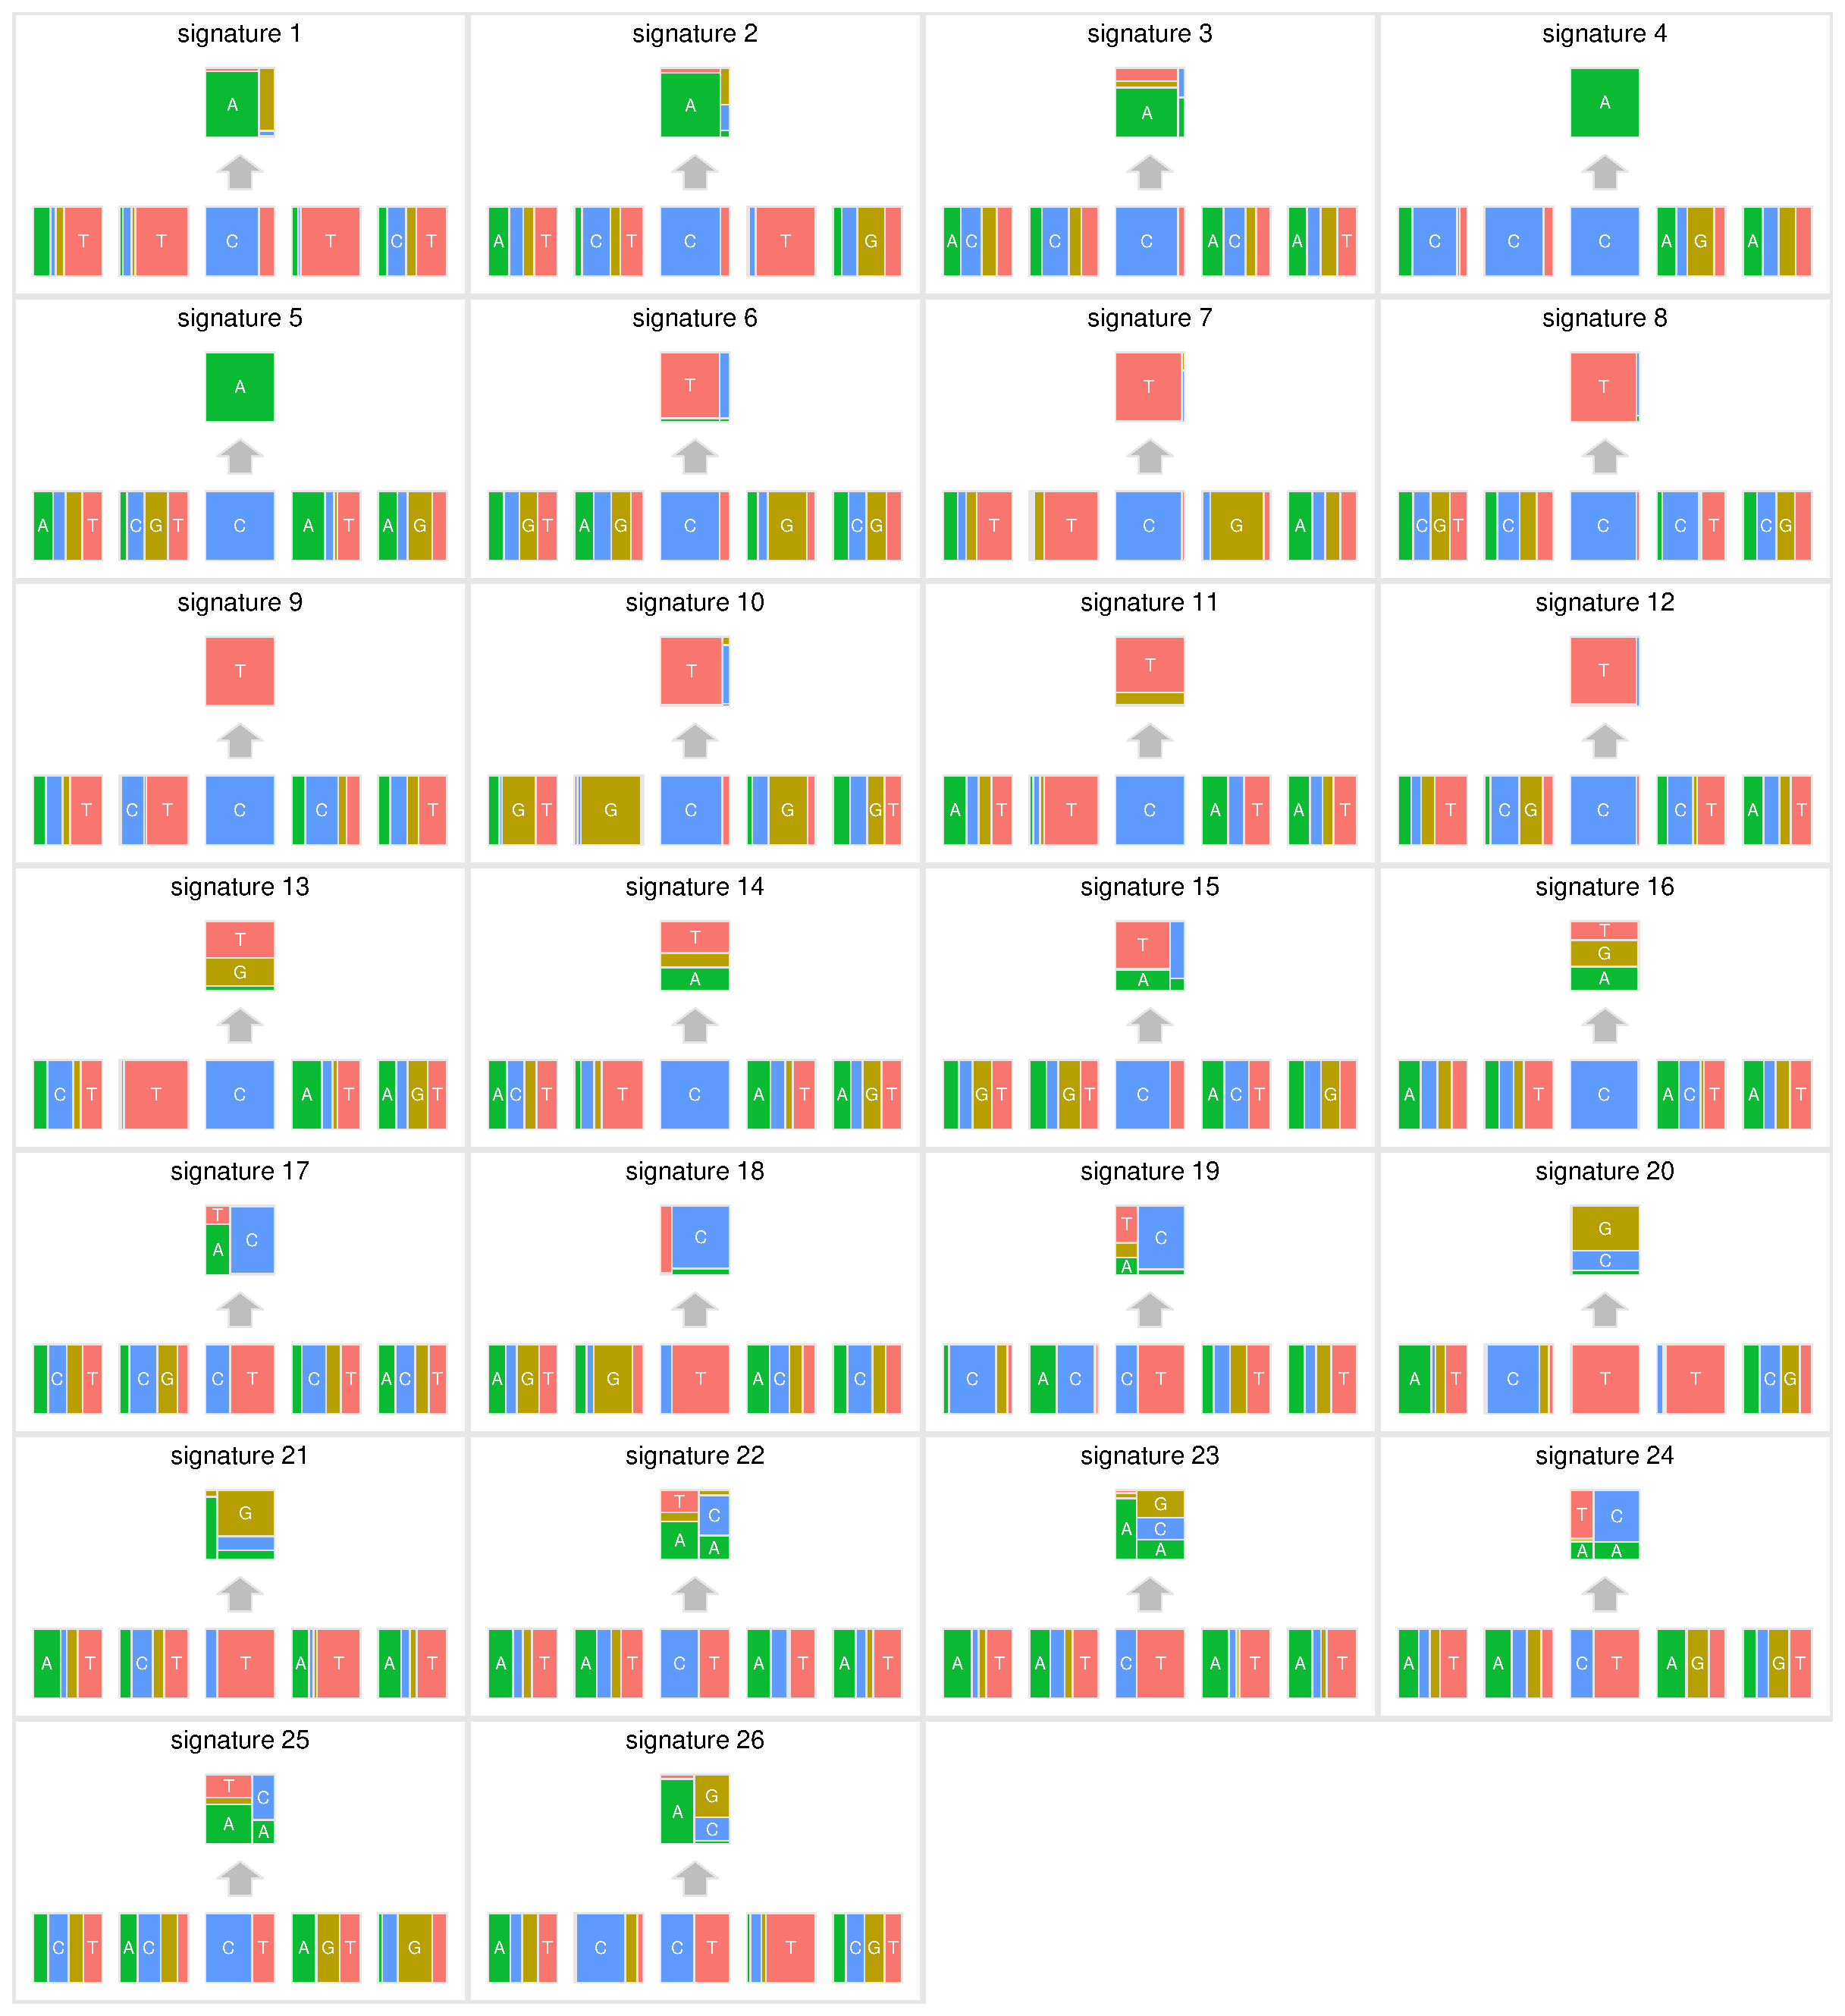
\includegraphics[width=16cm,height=17.5cm]{AlexandrovEtAl_mergedSignature.eps}
\caption{{\bf The summary of mutation signatures across 30 cancer types \cite{pmid23945592} obtained using the proposed method.}
Here, the substitution patterns and two 5' and 3' bases from the mutated sites are taken into account as mutation features.
First, mutation signatures were estimated separately in each cancer type, and then similar signatures were merged (see text).
}
\label{nature2013_sig_summary}
\end{figure}

\begin{figure}[h]
\centering
% 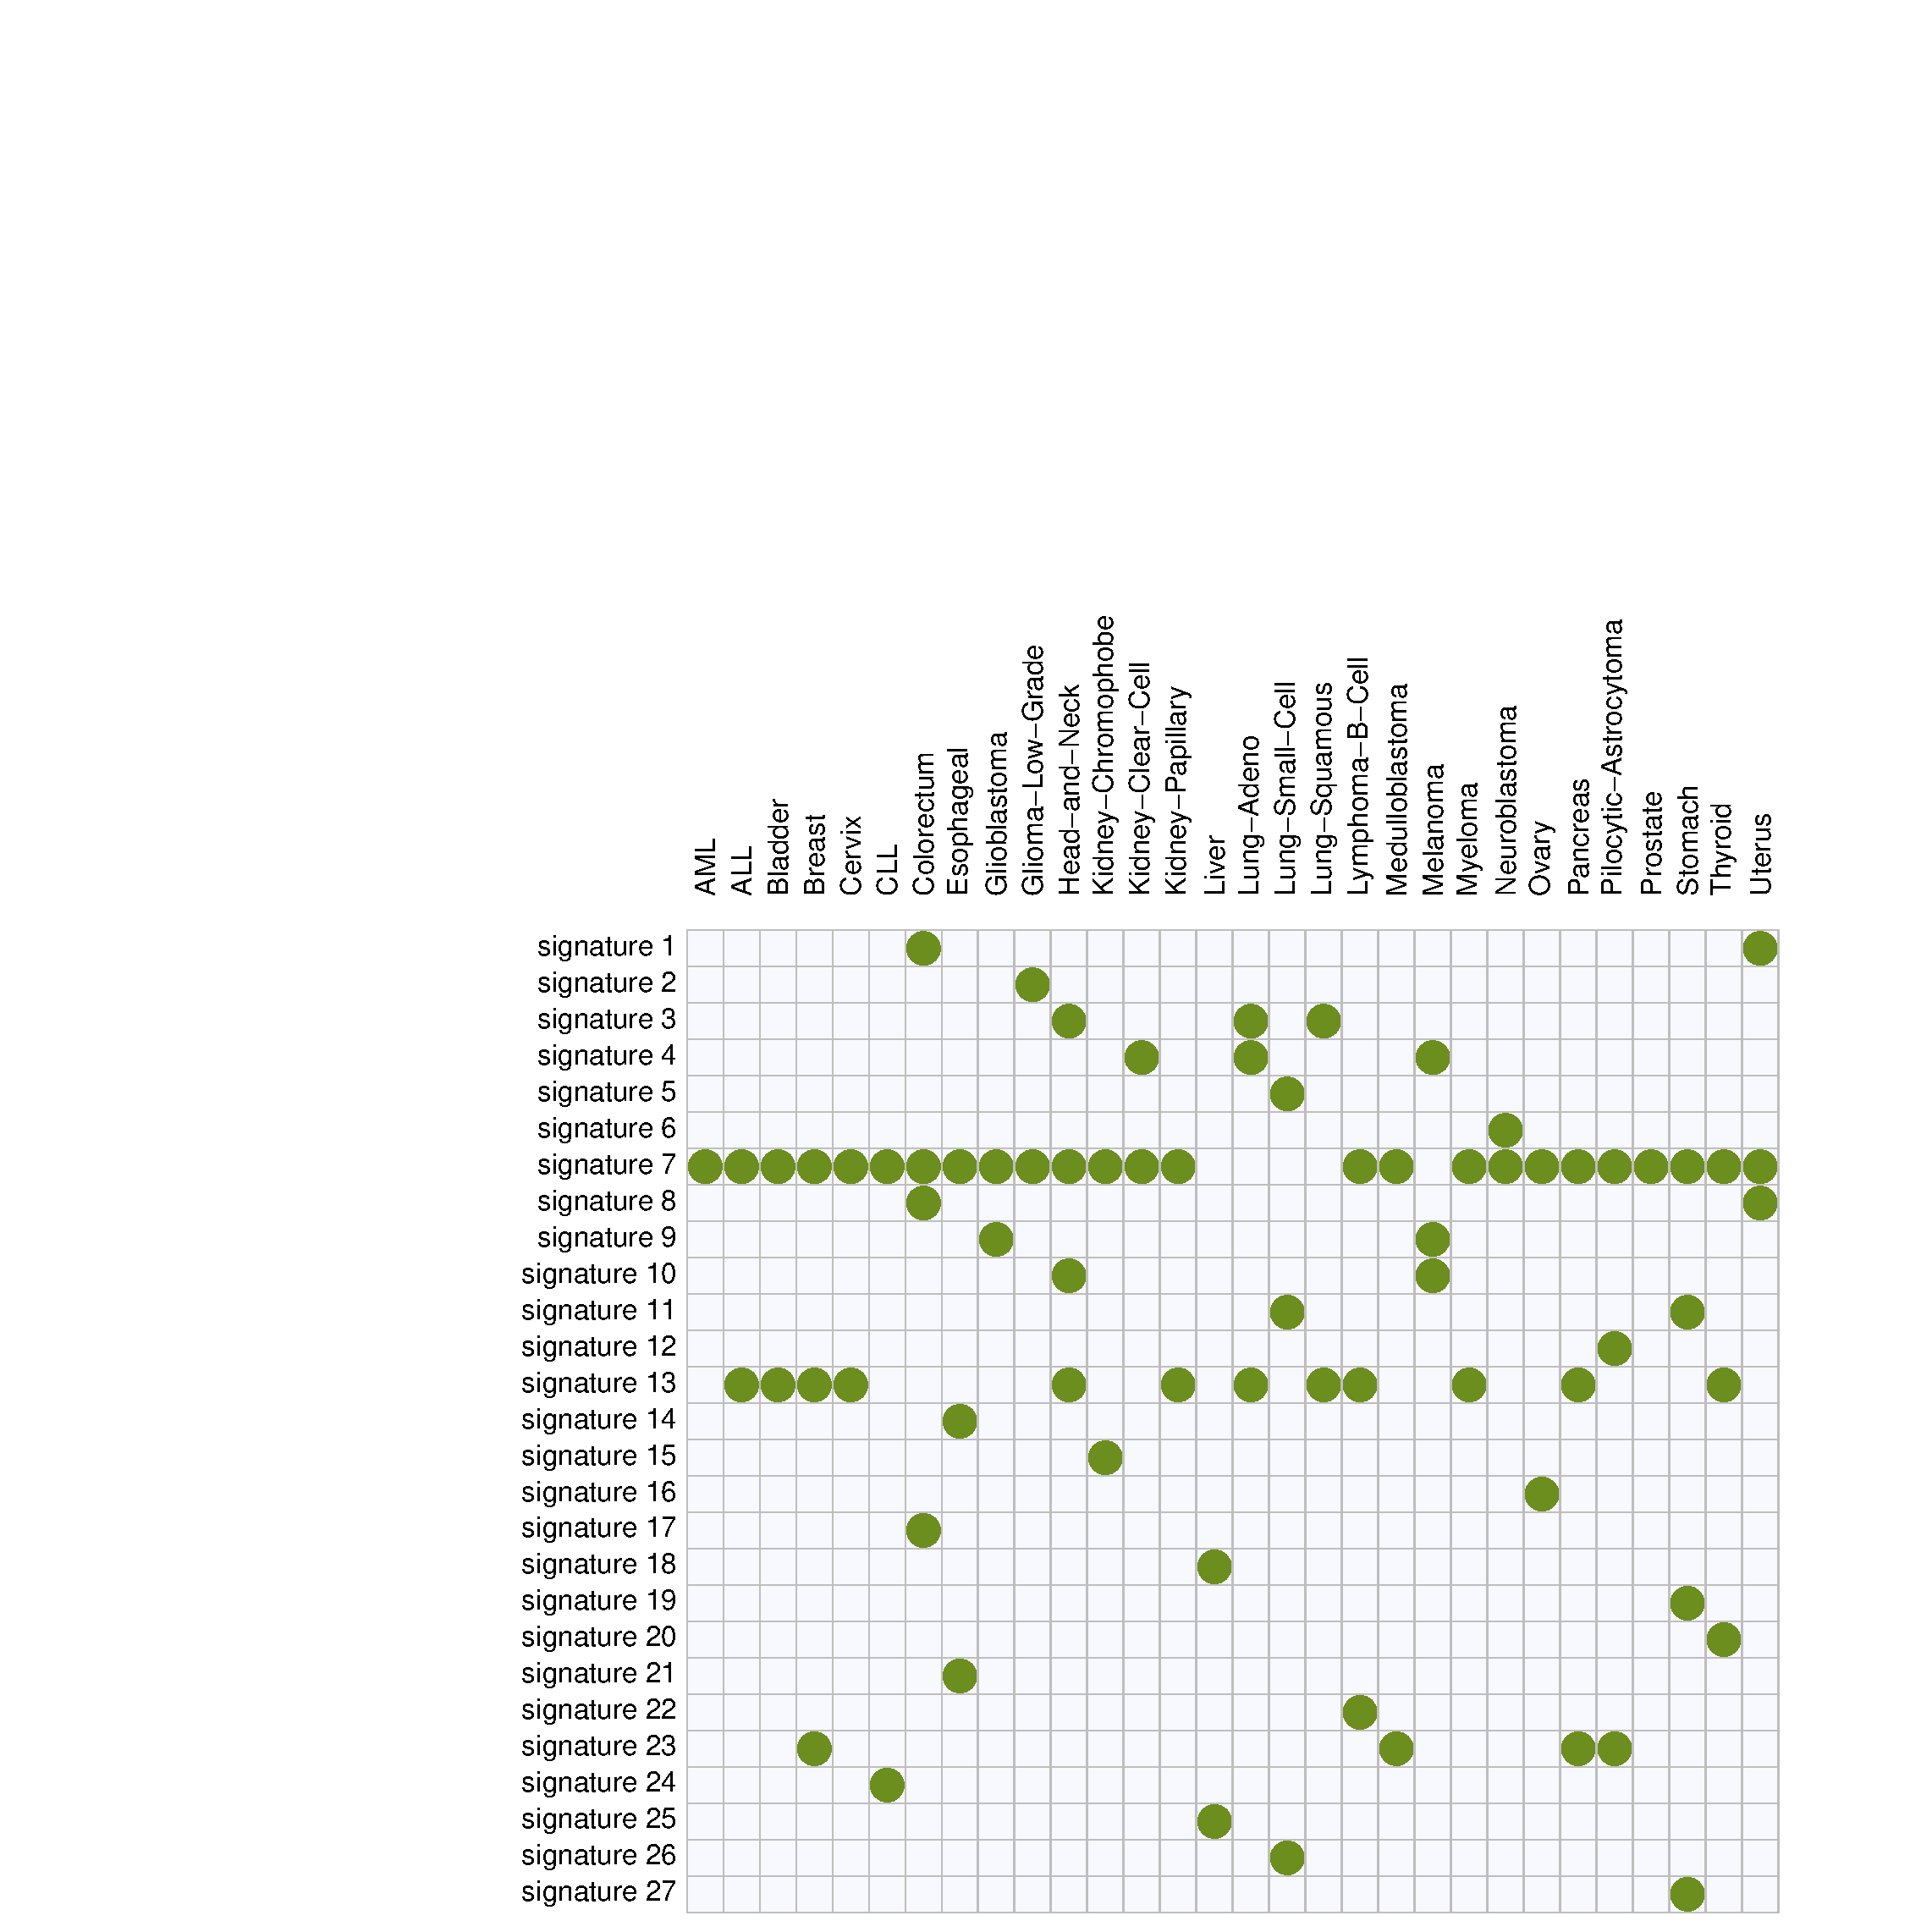
\includegraphics[width=15cm,height=15cm]{corrplot.eps}
\caption{{\bf The summary of membership of each mutation signature across 30 cancer types obtained using the proposed method.}}
\label{nature2013_sig_member}
\end{figure}



Signatures 1 and 8 (C $>$ A at TpCpT and C $>$ T at TpCpG, respectively) observed in colorectal and uterine cancers
appear likely to be associated with deregulated activity of the error-prone polymerase Pol $\epsilon$. 
In previous analyses of these data \cite{pmid23945592}, 
the signature for Pol $\epsilon$ dysfunction was represented by a single signature (their ``signature 10'').
In contrast our new approach uses two signatures.
Since these signatures are highly correlated,
and appear connected by
a single biological mechansim, we certainly do not argue
that inferring them as a single signature is ``wrong". However, splitting them into two signatures does help highlight certain features. Specifically,
signature 1 shows a transcription strand bias whereas signature 8 does not, and this is true for both colorectal and uterus cancers (Figs. S2C S2D).
This strand bias may be connected with the enrichment of 
C $>$A at TpCpT mutations in leading strands of replication forks
observed by \cite{pmid25228659}. Although replication strand bias is different from transcription strand bias, these two biases may be connected through the fact that replication origins prefer transcription start sites \cite{pmid23187890}.

These signatures also illustrate the ability of our model
to help highlight sequence context effects beyond the immediate flanking bases. Specifically, both signatures 1 and 8  show an elevated frequency of the T base at position $-2$,
and signature 1 also shows slightly elevated frequency of the T base at position $+2$
 (Figs. 6B, 6C ,S6C and S6D).
A previous study of Pol $\epsilon$  \cite{pmid25228659} 
found that a nonsense mutation R23X of TP53 is enriched in cancers with Pol $\epsilon$ defects.
In fact, the pattern of this mutation is C $>$ T at TpTpCpGpA, closely matching signature 8.
This illustrates that the inclusion of $\pm 2$ bases 
into signatures may be helpful for identifying underlying mechanisms.

\begin{figure}[h]
% \subfigure[APOBEC signature intensities at two 5' to the mutated site]{%
%   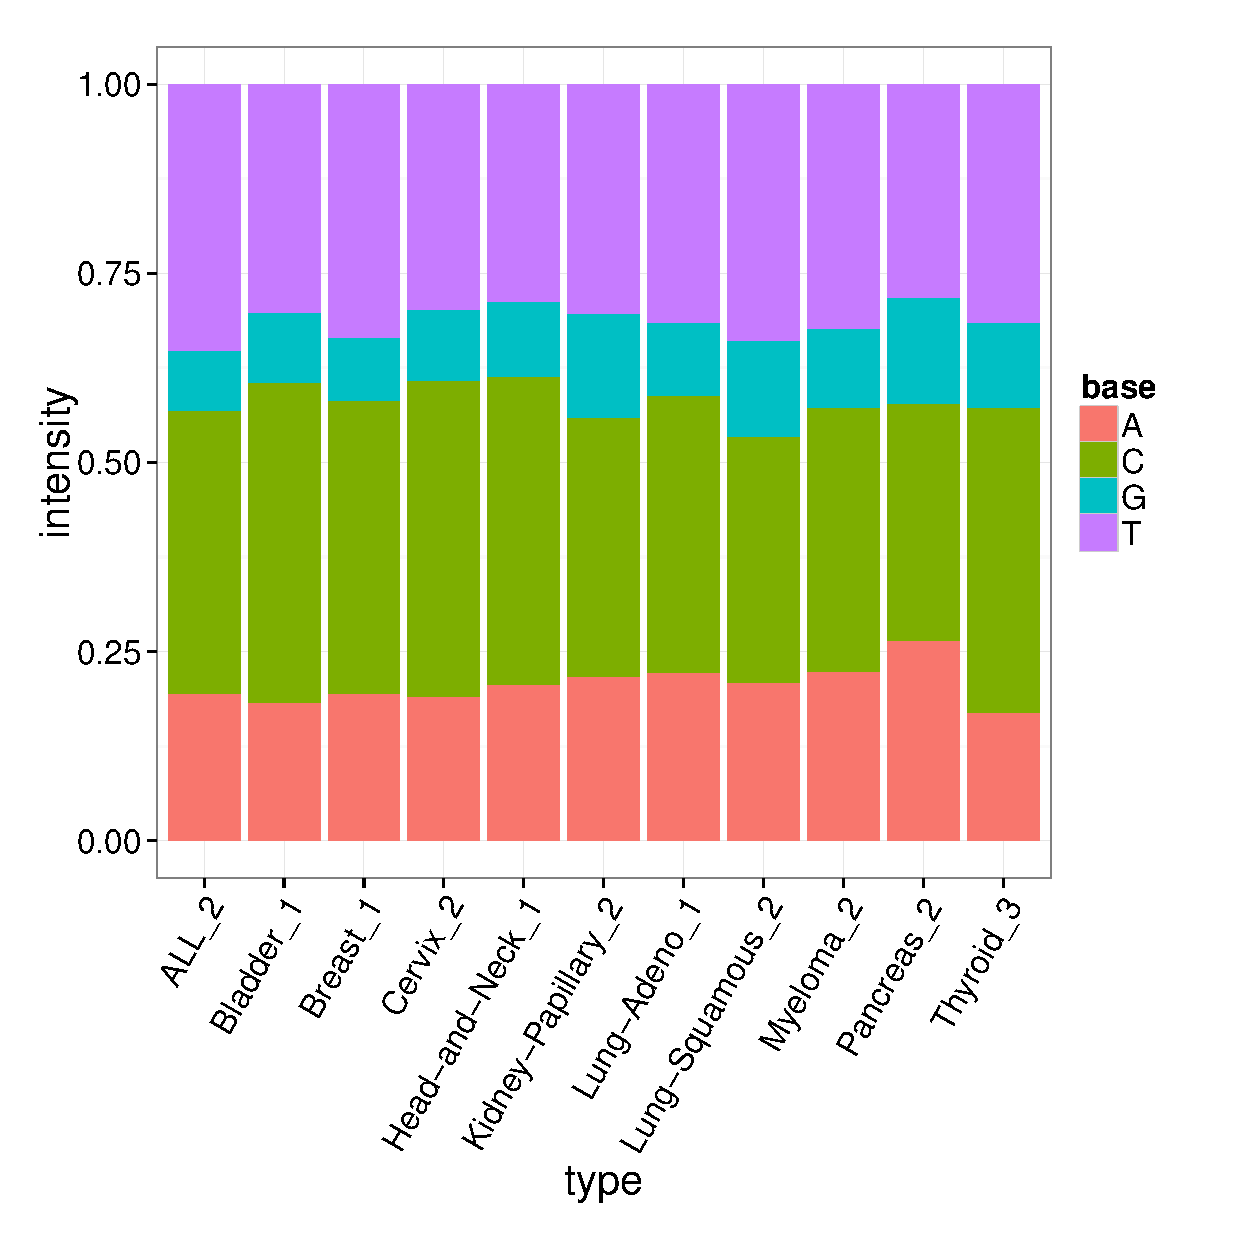
\includegraphics[width=14.5cm,height=6cm]{APOBEC_two5prime.eps}
%    \label{APOBEC_two5prime}}
% \subfigure[POLE1 signature intensities at two 5' to the mutated site]{%
%   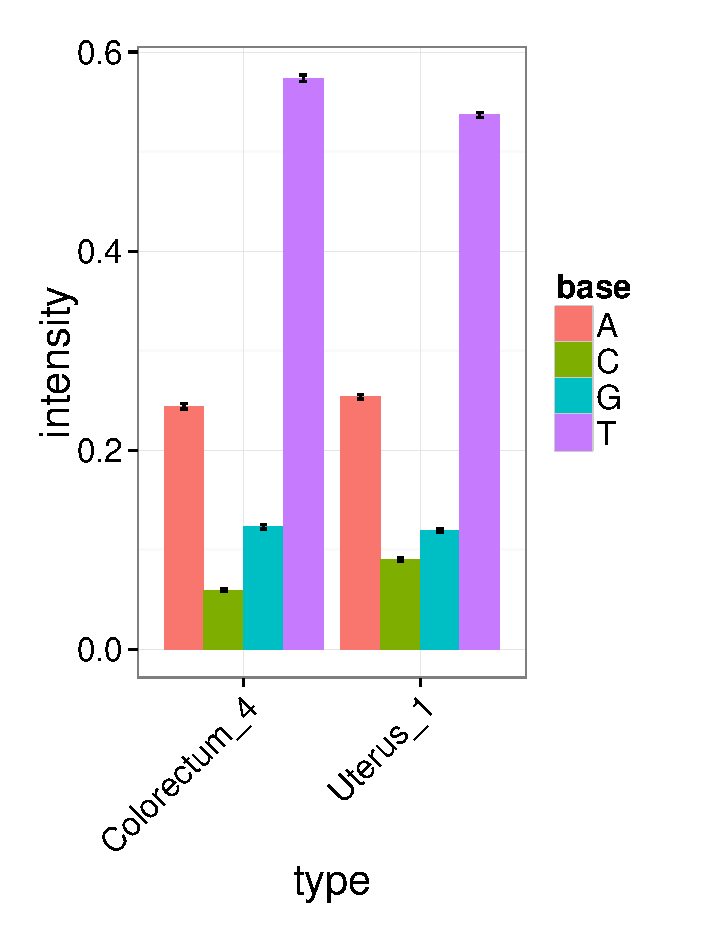
\includegraphics[width=4.5cm,height=6cm]{POLE1_two5prime.eps}
%   \label{POLE1_two5prime}}
% \quad
% \subfigure[POLE2 signature intensities at two 5' to the mutated site]{%
%   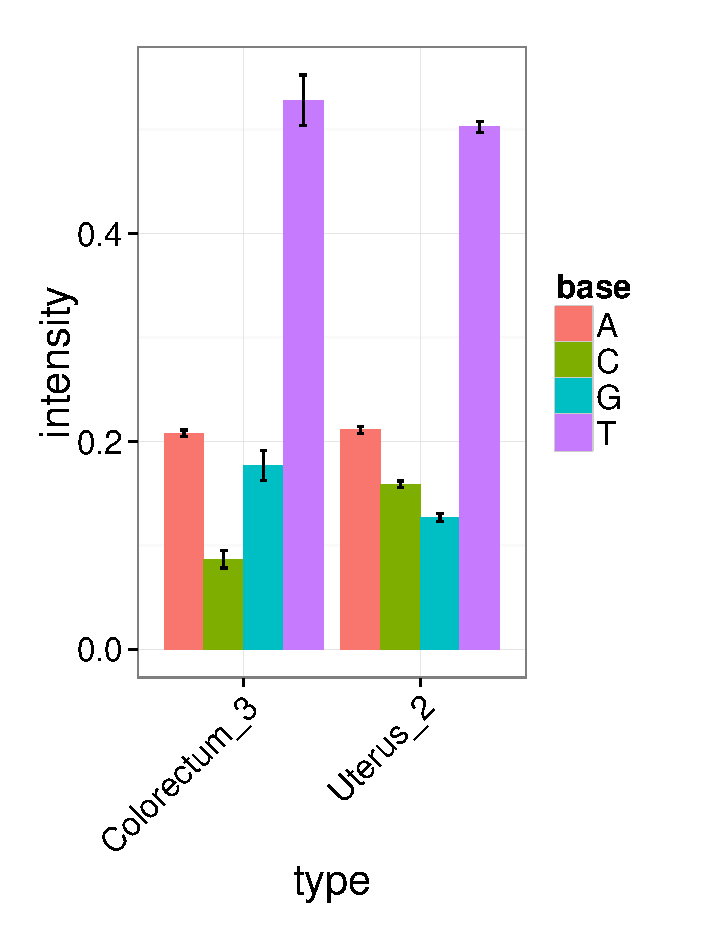
\includegraphics[width=4.5cm,height=6cm]{POLE2_two5prime.eps}
%   \label{POLE2_two5prime}}
% \subfigure[UV signature intensities at two 5' to the mutated site]{%
%   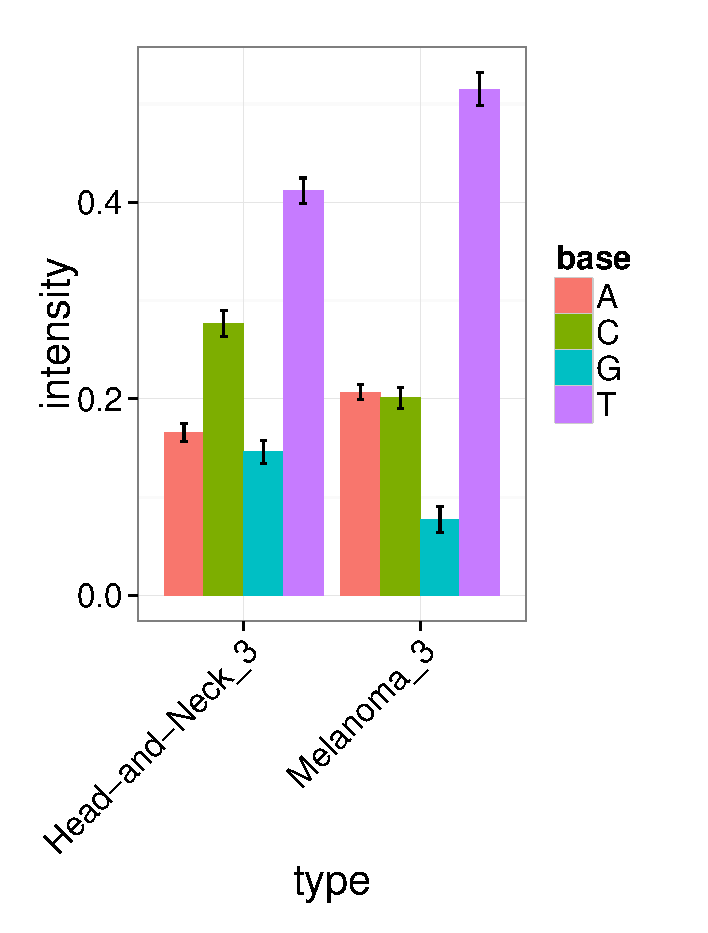
\includegraphics[width=4.5cm,height=6cm]{UV_two5prime.eps}
%   \label{UV_two5prime}}
% \quad
% \subfigure[The signature 11 intensities at two 5' to the mutated site]{%
%   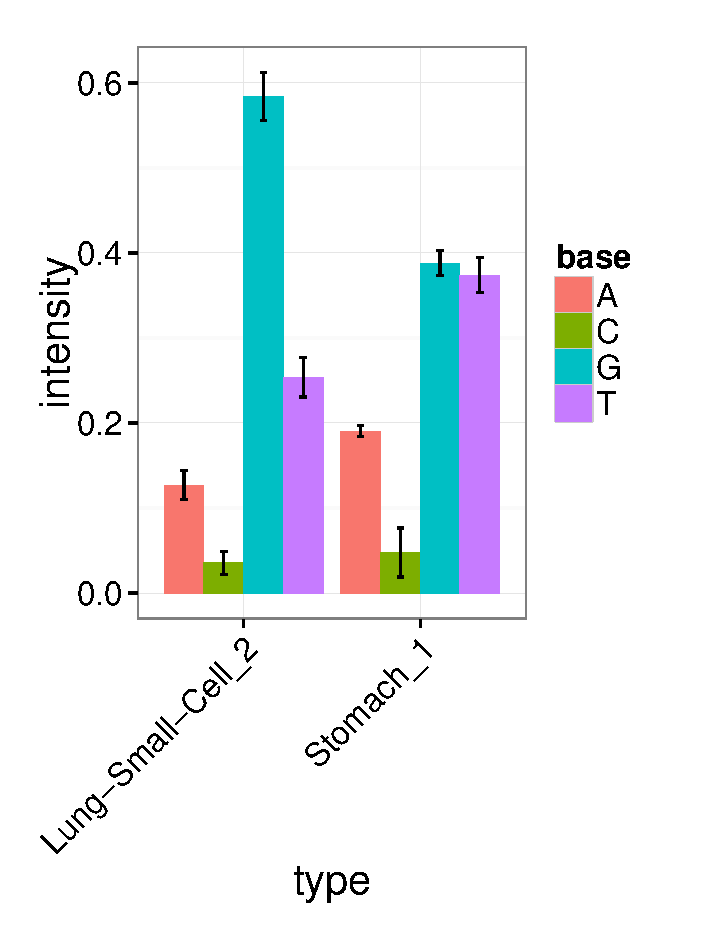
\includegraphics[width=4.5cm,height=6cm]{LMST_two5prime.eps}
%   \label{LMST_two5prime}}
\caption{{\bf The estimated frequencies of bases at two 5' to the mutated site for each cancer type.}
The bar heights show the estimated frequency for bases A, C, G and T at two 5' to the mutated site.
The error bars show bootstrapped standard errors.
(A, B, C, D, E) The intensities of signature 13 (APOBEC signature), signature 1 (the first POL $\epsilon$ signature),
signature 8 (the second POL $\epsilon$ signature), signature 10 (ultraviolet signature) and signature 11, respectively, at two 5' to the mutated site.
intensities at two 5' to the mutated site.
}
\label{two5prime}
\end{figure}

%XX Is the point here that looking $\pm 2$ bases can be useful and our method is particularly helpful here? XX

%XX this is important that it is drive by a single sample, but maybe just because yuichi looked more carefully and not new method XX
Signature 2 (C $>$ A at [CT]pCpT) is observed solely in low grade gliomas, and
appears related to, but slightly different from, the signature previously detected in the same cancer types (``signature 14'', \cite{pmid23318258}). 
Indeed, the corresponding signature in the previous study shows very complex patterns (C $>$ A at NpCpT or C $>$ T at GpTpN). Further investigation
revealed that this signature is driven by 
a single sample with an extremely high mutation rate (see Figs. S3A and S3B), and signature 2 disappeared when we removed this sample (see Fig. S4).
It may be that the complex low-grade-glioma specific signature detected in the previous study is driven by the same single sample.
We suggest that these signatures should be treated with caution until validated in additional samples. 
% XXX Need to discuss this wording and what it means XXX
 

%XX Also important, making a connection, but not the new method XX
Signature 4 (C $>$ A at CpCpG) observed in kidney clear cell carcinomas, lung adenocarcinomas and melanomas 
seems to correspond to the ``signature R2''  detected in the same cancer types (plus lung squamous carcinomas) in 
\cite{pmid23318258} (see their Supplementary Figures).
Again our analysis highlights additional contextual information, with a strikingly elevated frequency of base C at the $-2$ position (Figs. S5A, S5B and S5C).
However, for each cancer type, only a few samples support this signature (see Figs. S5D, S5E and S5F),
and the corresponding signature 
could not be validated in the previous study: most somatic mutations corresponding to that signature could not be validated by re-sequencing or visual inspection of BAM files using genomic viewers. Again, further investigation
yielded a potential explanation for this finding:
this signature largely matches that of a putative artifact caused by oxidation of DNA during acoustic shearing \cite{pmid23303777}, 
and we conclude that this signature, and the corresponding signature in previous work, are likely artefactual.
Although not of direct biological interest,
identifying artefactual signatures could be helpful in removing false positive mutations.

%XX highlights robustness of approach XX
Signature 13 (T $>$ [AGT] at TpCpN sites) was observed in 12 cancer types, and is surely related to the activity of the APOBEC family. The 12 inferred signatures are highly consistent among cancer types except for B-cell lymphoma (see Fig. S2A), highlighting the robustness
of our approach.  Almost all of them show enrichment of A and T and depletion of G base at the $-2$ position (Fig. 6A and S2A), 
consistent with the UCUT data above and previous analyses \cite{pmid23318258}.
The estimated transcribed strand specificities varied among cancer types, suggesting that there is not consistent strand-specificity in APOBEC signatures (and the observed variation may be due to estimation errors).
%Yuichi is that true?
Signatures 15 and 16 may also be related to APOBEC, although the estimated signatures are sufficiently different from 13 that they
were not merged into a single 
cluster by our specified clustering criteria.


Signatures 10, 11, 12, 19 and 21 provide further examples
of our method refining previously-observed signatures, highlighting strand biases and/or sequence context effects,
particularly 2 bases upstream of the substitution.
Signature 10 (C $>$T at [CT]pCpC) was observed in head and neck cancers and melanomas, and probably relates to ultraviolet light.
Consistent strand specificities among the two cancer types (Fig. S2E) matches previous results \cite{pmid23318258}, 
but our analysis additionally highlights elevated abundance of T at the $-2$ position (Figs. 6D and S2E). 
Signature 11 (C $>$ T at GpCp[CG]) appears in small-cell lung cancers and stomach cancers,
and seems to be the same as ``signature 15'' in the previous study, whose function remains unclear. Again our analysis highlights elevated abundance of G at the $-2$ position (Figs. 6E and S2F).
Signatures 12 (C $>$ T at [CG]pCp[CT]), 19 (T $>$ C at GpTpN) and 21 (T $>$ [CG] at CpTpT) observed in pilocytic astrocytomas, stomach cancers and oesophagus cancers, respectively, agree well with those detected in the same cancer types in the previous study \cite{pmid23318258}. However our analysis again refines these signatures,
highlighting a strand bias in all three, and sequence context effects at the -2 position in Signatures 12 and 21.
%although the causes of these signatures remain unknown.
%which should be validated by analysis of more samples from different cohorts and cancer types.


One signature, Signature 20, appears not to match any signatures in the previous analysis \cite{pmid23318258} and represents a potentially novel signature. 
This signature (T $>$ C at [AC]pTpN) is observed in thyroid cancers, and shows a very strong strand specificity, which could be due to transcription-coupled nucleotide excision repairs.
This signature may have been too weak for previous
methods to detect, perhaps because the mutation ratio of thyroid cancer is low, possibly reflecting improved sensitivity of our more parsimonious model.
%% download the TCGA data and check the visualization of the mutation position for this data.


The remaining signatures largely recapitulate previous results.
Signature 3 and 5 (C $>$ A at NpCpN) observed in head-and-neck cancers and three types of lung cancers are probably associated with tobacco smoking.
The estimated signature in each cancer type shows higher mutation prevalence on the template strand (Fig. S2B), 
which is consistent with the previous study \cite{pmid12379884, pmid23318258}.
Signature 6 (C $>$ A at NpCp[AT]) observed in neuroblastomas matches the pattern detected in the same cancer type in the previous study.
Signature 7 (C $>$ T at NpCpG sites) was observed in 25 out of 30 cancer type, and arguably relates to deamination of 5-methyl-cytosine.
Signature 9 (C $>$ T at NpCp[CT]) was observed in melanomas and glioblastomas, and is probably associated with a chemotherapy drug, temozolomide.
Signature 18 (T $>$ C at ApTp[AG]) observed in liver cancers has been shown to be more common in Asian cases than in other ancestries \cite{pmid25362482}, 
though the source of this signature is still not clear. 
In this signature, we observe a very strong strand specificity as shown in \cite{pmid25362482, pmid23318258},
suggesting a possible role for transcription-coupled nucleotide excision repairs.
 

%In summary, our method and analysis captures and refines 
%several previously observed mutation signatures, particularly
%detecting several novel characteristics at the $\pm 2$ position that are consistent across multiple cancer types.
%suggesting the existence of more hidden characteristics at the distant position from the mutated site.


\section*{Discussion}

In this paper, we presented new methods for inferring and visualizing mutation signatures from multiple cancer samples.
The new methods exploit simpler, more parsimonious, models
for mutation signatures than existing methods.
This improves stability of statistical estimation, and easily allows
a wider range of contextual factors (e.g. more flanking bases) to be
incorporated into the analysis. In addition, we provide a new
intuitive way to visualize the inferred signatures.

We have also emphasised the connection between mutation
signature detection, and the use of mixed-membership models
in other fields, particularly admixture analysis and document clustering.  This connection naturally raises the possibility of improving the proposed approach by learning from experiences in those other fields. For example, in admixture analysis, \cite{pmid12930761} found that the use of a correlated
prior on allele frequencies improved sensitivity to detect
population clusters; this suggests that it might be fruitful to consider a correlated prior distribution on signatures, to allow that some signatures - perhaps in different cancers - may be similar to one another (though not identical).
More generally, introducing certain prior distributions or penalty terms, such as sparsity-promoting penalties \cite{hoyer2004non, engelhardt2010analysis} and determinantal point process priors \cite{kulesza2012determinantal, kwok2012priors}
could improve both accuracy and interpretation.
Further, as the scale of cancer genome data becomes large,
more sophisticated computational approaches for estimating parameters may become necessary. We can potentially borrow a number of computational techniques such as those using EM-algorithm \cite{Hofmann:1999, tang2005estimation},
sequential quadratic programming \cite{zhou2011quasi}, Gibbs sampling \cite{pmid10835412,pmid14872004} 
and variational methods \cite{Blei:2003,teh2006collapsed,raj2014variational}.
Finally, to address the problem of determining the number of signatures, it may be fruitful to extend the framework to  
the Hierarchical Dirichlet processes \cite{teh2006hierarchical}.
% XX I think we should try to summarize the future work part from the methods more succinctly and put it here. XX
% yshira20150421 tried to summarize briefly as above

Although we have focused on point substitution mutations in this paper, 
many other types of mutations occur in cancer genomes, 
including insertions, deletions, double nucleotides substitutions, structural variations and copy number alterations \cite{meyerson2010advances, helleday2014mechanisms}.
Our framework could incorporate these additional mutation types, by 
summarizing them using appropriate mutation features.
In some cases, choice of appropriate features may need investigation. 
For example, longer deletions could be represented by the length of deletion and the adjacent bases; 
for short deletions (a few bases) it may be fruitful to include the actual deleted bases as part of the features.
%However, detailed investigation on what mutation features are practical is a future problem.

We have detected a number of mutation signatures having transcription strand biases, 
which are naturally considered to be associated with transcription activities.
Therefore, to further understand the effect of transcription activities on mutational mechanisms, 
we can include gene expression or RNA polymerase II occupancies to mutation features, 
so that the relationships of strand biases and transcription activities will be clarified.


Although we believe our new methods already provide
useful gains compared with existing approaches,
the methods are perhaps even more important for their future potential to incorporate other contextual data, including epigenetic data,
into mutation signature analysis. This is important, because
local mutation densities are closely related to a number of genomic and epigenetic factors, such as GC content, repeat sequences, chromatin accessibility and modifications, and replication timing \cite{pmid22820252, pmid21953857, pmid23422670, pmid23770567}.
A recent study found that epigenetic information in the cell types of origin of the corresponding tumors is the most predictive \cite{pmid25693567} for local mutation densities. A growing range of epigenetic data from many cell types are now available, and it will be interesting to integrate these epigenetic factors into mutation signature analysis to help understand how these epigenetic factors influence DNA damage and repair mechanisms. 
Our work here provides a straightforward way to do this: epigenetic
data can be simply added as features
to the mutation signature. 
We believe that 
the value and impact of our work, and 
specifically our proposed approach to modelling mutation signatures via independent features, will grow as more and more features
are incorporated into the analysis.







% In this paper, we have demonstrated that the independent representations could obtain more robust estimates than the full representations.
% Also, even in the independent representations, more complex mutational process could be represented by utilizing multiple mutation signatures.
% However, we still do not know about the exact mechanisms of mutational processes and 
% there might be those that should be represented by the full representations or somewhere between the full representations and the independent representations.
% We should keep exploring appropriate representations of mutation signature with expertise from biology and chemistry.

% You may title this section "Methods" or "Models". 
% "Models" is not a valid title for PLoS ONE authors. However, PLoS ONE
% authors may use "Analysis" 
\section*{Methods}


% Therefore, each probabilistic mutation signature, in general, consists of multiple multinomial distribution parameters.
% We give a way of visualizing probabilistic mutation signature (see Figure \ref{mutSig_example}), 
% which is reminiscent of sequencing logos \cite{pmid2172928}. 


\subsection*{Parameter Estimation}

The parameters $\{ \bm{f}_{k, l} \}$ and $\{ \bm{q}_i \}$
must be estimated from the available mutation data $\{ \bm{x}_{i,j} \}$. 
Here we adopt a simple approach that uses an EM-algorithm to maximise the likelihood. 

Let $g_{i, \bm{m}}$ denote the number of mutations in the $i$-th sample that have mutation feature vector $\bm{m}$.
In the E step of the EM algorithm, we calculate values of auxiliary variables $\theta_{i, k, \bm{m}}$ defined as
\begin{equation}
\theta_{i, k, \bm{m}} = \frac{  q_{i,k} \prod_{l=1}^L f_{k,l,m_l} }{ \sum_{k^{\prime} = 1}^K q_{i, k^{\prime} } \prod_{l=1}^L f_{k^{\prime}, l, m_l } }.
\end{equation}
Then, in the M-step, we update the parameters $\{ \bm{f}_{k, l} \}$ and $\{ q_{i, k} \}$ as
\begin{equation}
f_{k, l, p} = \frac{ \sum_{\bm{m} : m_l = p} g_{i, \bm{m}} \theta_{i, k, \bm{m}} }{ \sum_{p^{\prime} } 
\sum_{\bm{m} : m_l = p^{\prime}}  g_{i, \bm{m}}\theta_{i, k, \bm{m}} },
\end{equation}
\begin{equation}
q_{i, k} = \frac{ \sum_{\bm{m}} g_{i, \bm{m}} \theta_{i, k, \bm{m} } }{  \sum_{k^{\prime} }\sum_{\bm{m}} g_{i, \bm{m}} \theta_{i, k^{\prime}, \bm{m} } }.
\end{equation}

We use the R package SQUAREM \cite{varadhan2008simple} to accelerate
convergence of this EM algorithm (SQUAREM implements a general approach to accelerate the convergence of any fixed-point iterative scheme such as an EM algorithm).
To address potential problems with convergence to local minima,
we apply the EM algorithm several times (10 times in this paper) using different initial points,
and use the estimate with the largest log-likelihood.
See S3 Text for the derivation of the above updating procedures.


\subsection*{Background signatures}

% The intrinsic composition of genome sequence may 
% influence the estimated mutation signatures.
% For example, the number of observed C $>$ T transitions at CpG sites may increase at promoter regions,
% just because CpG dinucleotides are more frequent in those regions.
% In previous work \cite{pmid23628380}, this background problem was dealt by explicitly incorporating mutation ``opportunity'' coefficients into the model.

% XX This is not quite clear to me. Also may need including in Main text? XX

% Here, to offset the influences of intrinsic sequence composition, we add background signatures 
% $\{ \bm{f}_{0, \bm{m}} \} \in \Delta^{M_1 \times \cdots \times M_L}$.
% For example, when obtaining the background signatures in case of considering substitution patterns and up to $\pm 2$ flanking bases, 
Here, we describe how the background mutation signature is 
obtained in the case where mutation features are the substitution patterns, the $\pm 2$ flanking bases, and the transcription strand.
Since the majority of the data used in this paper is exome sequencing data, and since we consider transcription strand as a mutation feature,
we use the exonic regions of the human genome reference sequence to obtain the background mutation signature.
First we calculate the frequencies of 5-mers with transcription strands of the corresponding exon,
where we take complement sequences and flip the strand for those whose central bases are A or G.
Then, assuming alternated bases are equally likely from each central base C and T, 
the frequency of each mutation feature is derived directly from those of the 5-mers and transcription strands.
Finally, the probability of each mutation feature is derived by normalizing each frequency to sum to one.



\subsection*{Estimating standard errors}

We use the non-parametric bootstrap \cite{efron1994introduction} to calculate standard errors for parameter estimates. This involves resampling somatic mutations from the empirical distribution of the original data $\{ \bm{x}_{i,j} \}$ for each cancer genome. For each of 100 such bootstrap samples, we re-fitted the model, using parameters obtained for the original data as initial points.
We then used sample standard errors of the inferred mutational signatures as estimates of parameter standard errors.


\subsection*{Selecting the number of signatures}

Determining an appropriate number of mutation signatures $K$ is a challenging task. 
One approach is to utilize some statistical information criteria such as AIC \cite{akaike1974new} or BIC \cite{schwarz1978estimating}.
In the population structure problems, for example, 
the Bayesian deviance \cite{pmid10835412} 
and cross-validation \cite{alexander2011enhancements} have been suggested.
One previous study on mutation signature problems \cite{pmid23628380} utilized BIC.
On the other hand, the problem of using these statistical information criteria is that most of them are based on the likelihood,
where slight deviations between the specified probabilistic models and the reality sometimes leads to additional
(possibly spurious) mutation signatures being selected to
compensate for those deviations.

In this paper, instead of utilizing a statistical information criteria, we adopt the following strategy:
\begin{itemize}
\item
After calculating the likelihood and standard errors of parameters for a range of $K$,
the value of $K$ is determined at the point where the likelihood is sufficiently high, 
and the standard errors are sufficiently low \cite{pmid23318258}.

\item
When, for $k_1$-th and $k_2$-th mutation signatures, 
we could detect strong correlations between the estimated membership parameters 
for each cancer genome
($(q_{1,k_1}, q_{2,k_1}, \cdots, q_{I,k_1})$ and $(q_{1,k_2}, q_{2,k_2}, \cdots, q_{I,k_2})$),
and the two mutation signatures ($\{ \bm{F}_{k_1} \}$ and $\{ \bm{F}_{k_2} \}$) show similar patterns,
then this suggests that the method may have split one mutation signature into two. We choose $K$ to be small enough that such pairs of mutation signatures do not occur.
\end{itemize}

These strategies are not claimed as optimal, but appeared
to  provide satisfactory results in our applications here.
The development of automated and practical approaches for choosing $K$ is a possible area for future development.


\subsection*{Existing methods as a special case}

Previous approaches to mutation signature modelling in \cite{pmid23945592, pmid23318258} are a special case of our framework. Specifically, they correspond to combining
all possible combinations of mutation features into a single ``meta-feature'', which takes $M_1 \times M_2 \times \dots \times M_L$ possible values.
Thus, instead of having $L$ features with $\bm{M} = (M_1,\dots,M_L)$,
existing approaches have one feature with $\bm{M} = (M_1 \times \dots \times M_L)$ (see S1 Table). 
The resulting model allows for arbitrary distributions on the $M_1 \times \dots \times M_L$
feature space, and we call the resulting model the ``full model''.
The full model can represent complicated dependencies in a single
signature. For example,
a situation where C $>$ A is frequent at ApCpG sites and C $>$ T is frequent at TpCpA sites could be represented with one signature.
This may be desirable in some settings and not in others.
However, when many mutation contextual factors are taken into account and the number of free parameters becomes huge,
estimated results can be unstable and unreliable.
Furthermore, there is a risk of over-interpreting the complex features of estimated signatures.




\subsection*{Relationship with mixed-membership models}

Our model is closely related to
mixed-membership models that have been adopted in other applications, 
such as document classification and population structure inference problems. 
In this subsection, we outline these relationships,
slightly abusing notation to contrast the relationships. 

In the topic model \cite{Hofmann:1999,Blei:2003},
which are a form of mixed-membership models frequently used in document classification problems,
each document is assumed to have $K$ different ``topics'' in varying proportions ($\bm{q}_i \in \Delta^K$),
where each topic is characterized by a word frequency (a multinomial distribution on a set of words $W$ ($\bm{f}_k \in \Delta^W$).
And each word is assumed to be generated by one of $K$ multinomial distributions (topics).
The detailed generative process of the $j$-th word in the $i$-th document $x_{i,j}$ is:  
\begin{enumerate}
\item
Generate the underlying topic for the $j$-th word: $z_{i,j} \sim \text{Multinomial} (\bm{q}_i)$, where $z_{i,j} \in \{1,\cdots,K \}$.
\item
Generate $x_{i,j} \sim \text{Multinomial} (\bm{f}_{z_{i,j}})$, where $x_{i,j} \in \{1, \cdots, W \}$.
\end{enumerate}
Actually our ``full model'' ($L=1$) is essentially the same as a topic model. 

On the other hand, in population structure inference problems \cite{pmid10835412, pmid19648217}, 
each individual is assumed to be an admixture of $K$ ancestries in varying proportions, 
where each ancestry is characterized by the allele frequency at each SNP locus.
Each SNP genotype of an individual is assumed to be generated by the two step model:
first, an ancestry (``population") is chosen according to the admixture proportion for each individual,
and then the SNP genotype is generated according to the allele frequency of the selected ancestry at that locus.
The relationships among the mutation signature models, topic models and population structure models are summarized in Table \ref{tab_pop}.


\begin{table}[!ht]
\begin{adjustwidth}{-2.25in}{0in} % Comment out/remove adjustwidth environment if table fits in text column.
\caption{
{\bf Relationships among mutation signature model, topic models, and population structure models.}
}
\begin{tabular}{|l|l|l|l|} \hline
problem & $\bm{x}_{i,j}$ & $\bm{f}_{k}$ & $\bm{q}_{i}$  \\ \hline
mutation signature model & the $j$-th mutation  & the feature dist.  & the signature dist.  \\
& in the $i$-th cancer genome & for the $k$-th signature & for the $i$-th cancer genome \\ \hline
topic model &  the $j$-th word & the word dist. & the topic dist. \\ 
& in the $i$-th document & for the $k$-th topic & for the $i$-th document \\ \hline
population structure model & the $j$-th locus genotype & the allele freq.  & the admixture dist. \\
& of the individual $i$  & for the ancestry $k$ & for the individual $i$ \\
\hline 
\end{tabular}
\label{tab_pop}
\end{adjustwidth}
\end{table}


As pointed out by \cite{ding2008equivalence}, there is a  close relationships between mixed-membership models and nonnegative matrix factorization,
which has been successfully used in the previous studies for mutational signature problems \cite{pmid22608084, pmid23318258, pmid23945592}.
In fact, the proposed method can be seen as non-negative matrix factorization with additional restrictions.
See S4 Text for details of the relationship between the proposed approach and nonnegative matrix factorization.



\section*{Supporting Information}
\subsection*{S1 Text}
\label{simulation}
{\bf Experiments on synthetic data.}

\subsection*{S2 Text}
\label{UCUT_supp}
{\bf Experiment on UCUT data with the various number of mutation signatures.}

\subsection*{S3 Text}
\label{EM_math}
{\bf Derivation of EM algorithm.}

\subsection*{S4 Text}
\label{NMF_math}
{\bf Relationship with nonnegative matrix factorization.}

\subsection*{S1 Table}
\label{mfexample}
{\bf Example of representation for mutation patterns (substitution patterns and one 5' and 3' bases).}
In the independent representation, the elements of vector show substitution patterns, 5' adjacent bases and 3' adjacent bases, respectively.
For substitution pattens, 1 to 6 values are assigned to C$>$A, C$>$G, C$>$T, T$>$A, T$>$C and T$>$G in this order.
For 5' and 3' adjacent bases, 1 to 4 values are assigned to A, C, G and T.
Note that the original base is fixed to C or T to remove the redundancy of complement sequences.

\subsection*{S2 Table}
\label{nature2013_sigNum}
{\bf The number of mutation signatures selected for each cancer type for each cancer type in the Alexandrov et al. (2013) data.}

\subsection*{S1 Figure}
\label{UCUT_APOBEC_twoFivePrime}
{\bf The frequencies of bases at two 5' to the mutated site for the APOBEC mutation signatures obtained in UCUT data using the independent and full models.}

\subsection*{S2 Figure}
\label{nature2013_sig_list}
{\bf The list of several signatures extracted in each cancer type in the Alexandrov et al. (2013) data.}
(A) APOBEC signatures (signature 13) obtained in each cancer type.
(B) Smoking signature in each cancer type.
(C) The first Pol $\epsilon$ signature (signature 1)  in each cancer type.
(D) The second Pol $\epsilon$ signature (signature 8) in each cancer type.
(E) The ultraviolet signature i(signature 10) n each cancer type.
(F) Unknown signature (signature 11) obtained in lung small cell carcinomas and stomach cancers.


\subsection*{S3 Figure}
\label{LGG_membership}
{\bf The estimated membership parameters of low grade gliomas.}
(A, B) Estimated membership parameter by the proposed method in normal and log scale.
We have selected top 100 cancer samples according to the number of mutation.
The height of bar shows (the logarithm of) the number of mutations for each sample,
and the ratio of colored division shows the ratio of estimated membership parameters for each signature and sample.
The low grade glioma specific signature detected by the proposed method is the signature 2.
We can see that the mutations corresponding to signature 2 is mostly from the sample with an extremely high mutation rate.


\subsection*{S4 Figure}
\label{LGG_signatures}
{\bf The signatures obtained for the original data and for the data without the hyper-mutated case.}
(A) The result for the original data ($K = 3$). The first (from the left) signature seems to be one from deamination of 5-methyl-cytosine. 
The second signature is the low grade glioma signature.
(B, C, D, E) The result for the data without the hyper-mutated sample for $K = 2, 3, 4$ and $5$, respectively.
Although the signature related to deamination of 5-methyl-cytosine remained, low grade glioma specific signature could not be observed.

\subsection*{S5 Figure}
\label{oxidation}
{\bf The putative oxidative artifact signatures and membership parameters estimated for each cancer.}
(A) The second signature detected in kidney clear cell carcinomas.
(B) The first signature detected in lung adenocarcinomas.
(C) The first signature detected in melanomas
(D, E, F) Estimated membership parameter for kidney clear cell carcinomas, lung adenocarcinomas and melanomas, respectively.
For each cancer type, 
We have selected top 100 cancer samples according to the number of mutation.
The height of bar shows the number of mutations for each sample,
and the ratio of colored division shows the ratio of estimated membership parameters for each signature and sample.
We can see that the signature corresponding to putative oxidative artifacts concentrates on a small number of samples.

\section*{Acknowledgments}

We thank to Dr. Daichi Mochihashi for helpful discussion and comments on an earlier version of the method;
Dr. Hiromichi Suzuki for many helpful feedback on the R packages;
Dr. Ziyue Gao for reading the manuscript and providing many helpful comments.

This project was deeply influenced by the broader intellectual and academic environment surrounding Matthew Stephens's Laboratory,
when the first author stayed at the University of Chicago as a visiting scholar. The first author thanks Dr. John Novembre,
Dr. Jacob Degner and all the members of Matthew Stephens and John Novembre Laboratories for helpful discussion and comments.


\nolinenumbers

% \section*{References}

% Either type in your references using
% \begin{thebibliography}{}
% \bibitem{}
% Text
% \end{thebibliography}
%
% OR
%
% Compile your BiBTeX database using our plos2009.bst
% style file and paste the contents of your .bbl file
% here.
% 

% \bibliographystyle{plos2009}

\bibliography{plos_template}





\end{document}